% !TeX encoding = utf8
% !TeX spellcheck = en_US
% !BIB program = biber
% !TeX program = lualatex


\documentclass[12pt,oneside,letterpaper]{article}

\nonstopmode

% Set a better default text area (note: don't use this and geometry at the same time.)
% \usepackage[DIV=10]{typearea}
\usepackage[margin=1.5in]{geometry}
\usepackage{fontspec}
\defaultfontfeatures{Ligatures=TeX}
\usepackage{amsmath}  % must be loaded before unicode-math
\usepackage{amsthm}
% Libertinus code suggested by https://tex.stackexchange.com/a/364502
\usepackage[
    math-style=ISO,
    bold-style=ISO,
    partial=upright,
    nabla=upright
]{unicode-math}
\setmainfont[Numbers={OldStyle, Proportional}]{Libertinus Serif}
\setsansfont{Libertinus Sans}
\setmathfont{Libertinus Math}
\newfontface\titlefont{Libertinus Serif Display}[Numbers={OldStyle, Proportional}, Fractions=Off,Ligatures=Common]
\newfontface\textfracfont{Libertinus Serif}[Numbers={OldStyle, Proportional}, Fractions=On]
\newfontface\tabularoldstylefont{Libertinus Serif}[Numbers={OldStyle, Monospaced}, Fractions=Off]

\usepackage{csquotes}
\usepackage[final]{microtype}
\frenchspacing{}
\microtypecontext{spacing=french}

% Don't do ligatures in compound words:
\usepackage[english]{selnolig}

\usepackage{ragged2e}  % allow for ragged-right with hyphenation


% Format sections:
% \titleformat{command}[shape]{format}{label}{sep}{before-code}[after-code]
\usepackage[it, small]{titlesec}

% Format itemized lists
\usepackage{enumitem}
\setlist{nolistsep} % more aggressive than noitemsep

% allow page breaks in math equations
\allowdisplaybreaks

\newcounter{axiomcounter}
\newcounter{theoremcounter}
\newcounter{examplecounter}
\newcounter{propositioncounter}
\newcounter{lemmacounter}
\newcounter{corollarycounter}

% Make it easier to change the spacing around these math environments
\newlength{\premathenv}
\setlength{\premathenv}{0.2\baselineskip}
\newlength{\withinmathenv}
\setlength{\withinmathenv}{0\baselineskip}
\newlength{\postmathenv}
\setlength{\postmathenv}{\premathenv} % default to the same, but could change.


\newcommand{\norm}[1]{\left\lVert#1\right\rVert}
\newcommand{\length}[1]{\left\lvert#1\right\rvert}

\theoremstyle{definition}
\newenvironment{theorem}[1]{%
\vspace{\premathenv}%
\refstepcounter{theoremcounter}%
\noindent\textbf{Theorem \thetheoremcounter}
{#1}
\vspace{\withinmathenv}
}{% end of beginning of environment, beginning of end of env
\vspace{\postmathenv}%
}
\newenvironment{proposition}[1]{%
\vspace{\premathenv}%
\refstepcounter{propositioncounter}%
\noindent\textbf{Proposition \thepropositioncounter}
{#1}
\vspace{\withinmathenv}
}{% end of beginning of environment, beginning of end of env
\vspace{\postmathenv}%%
}
\newenvironment{lemma}[1]{%
\vspace{\premathenv}%
\refstepcounter{lemmacounter}%
\noindent\textbf{Lemma \thelemmacounter}
{#1}
\vspace{\withinmathenv}
}{% end of beginning of environment, beginning of end of env
\vspace{\postmathenv}%
}
\newenvironment{corollary}[1]{%
\vspace{\premathenv}%
\refstepcounter{corollarycounter}%
\noindent\textbf{Corollary \thecorollarycounter}
{#1}
\vspace{\withinmathenv}
}{% end of beginning of environment, beginning of end of env
\vspace{\postmathenv}%
}
\newenvironment{axiom}[1]{%
\vspace{\premathenv}%
\refstepcounter{axiomcounter}%
\noindent\textbf{Axiom \theaxiomcounter}
{#1}
\vspace{\withinmathenv}
}{% end of beginning of environment, beginning of end of env
\vspace{\postmathenv}%
}
\newenvironment{example}[1]{%
\vspace{\premathenv}%
\refstepcounter{examplecounter}%
\noindent\textbf{EXAMPLE \theexamplecounter}
{#1}
\vspace{\withinmathenv}
}{% end of beginning of environment, beginning of end of env
\vspace{\postmathenv}%
}

\renewenvironment{proof}{%
\vspace{\premathenv}% previously \vspace{1\baselineskip}
\noindent{\textit{Proof:} }
}{% end of beginning of environment, beginning of end of env
\qed
\vspace{\postmathenv}% previously \vspace{1\baselineskip}
}
\newtheorem{case}{Case}
\renewcommand*{\thecase}{\Alph{case}}
\newtheorem{assumption}{Assumption}
\renewcommand*{\theassumption}{\Alph{assumption}}

\def\equationautorefname~#1\null{(#1)\null}

\newcounter{auditpolicy}
\setcounter{auditpolicy}{-1}
\newenvironment{auditpolicy}[1]{%
\refstepcounter{auditpolicy}%
{\tabularoldstylefont(\theauditpolicy)}~#1%
}


\usepackage{fancyhdr}
\pagestyle{fancy}
\lhead{}
\chead{}
\rhead{}
\lfoot{}
\cfoot{}
\rfoot{\thepage}
\renewcommand{\headrulewidth}{0pt}
\usepackage{xcolor}

% Redefine \left and \right with better spacing
\usepackage{mleftright}
\mleftright{}

% Define \expected and \indicator commands
\DeclareMathOperator{\blackboardE}{\mathbb{E}}
\newcommand{\expected}[1]{\blackboardE\left[#1\right]}
\newcommand{\indicator}[1]{\symbf{1}\left[#1\right]}



\usepackage{rotating} % provide the sidewaysfigure environment

% Set up tables
\usepackage[online,flushleft]{threeparttable}
\usepackage{dcolumn}
\newcolumntype{d}{D{@}{\hspace{0pt}}{4}}
\newcommand{\textcol}[1]{\multicolumn{1}{c}{#1}}

% \usepackage{sparklines}
\usepackage{tabularx}
\usepackage{longtable}
\usepackage{booktabs}

% Bibliography
\usepackage[
  authordate,
  isbn=false,
  backend=biber,
  autopunct=true,
  uniquename=false
  % backref=true
]{biblatex-chicago}
\renewcommand*{\bibfont}{\small}
\addbibresource{refs.bib}
\addbibresource{data_cites.bib}
\addbibresource{methane_measurement_refs.bib}

% use the \ce{} command for chemistry expressions like \ce{CO2}
\usepackage[version=4]{mhchem}

\usepackage{nameref}

% Set up a boolean so we can easily turn endfloat on and off.
% To turn on, change to \setboolean{endfloat}{true}
\usepackage{ifthen}

\newboolean{endfloat}
\setboolean{endfloat}{false}
\ifthenelse{\boolean{endfloat}}{
  \usepackage{endfloat}
  % stopendfloat from putting everything on separate pages
  \renewcommand{\efloatseparator}{\mbox{}}
}{ % else :
  \usepackage{placeins} % provide \FloatBarrier command
}

\usepackage{graphicx}
\graphicspath{{../graphics/}}
\usepackage{import} % better relative import paths
\usepackage{tikz}
\usetikzlibrary{calc}
\usepackage{wrapfig} % provides wrapfigure and wraptable environments


% Define a command \blfootnote (blind foodnote or blank footnote)
% Redefine \thefootnote to remove the symbol
% Redefine \@makefntext to try to mimic the biblatex-chicago option footmarkoff, but only for the scope of this command.
% Then reset the counter.
\makeatletter
\newcommand{\blfootnote}[1]{%
  \begingroup
  \renewcommand{\thefootnote}{}%
  \renewcommand{\@makefntext}{}%
  \footnote{#1}%
  \addtocounter{footnote}{-1}%
  \endgroup
}
\makeatother


% Add an orcid logo:
% Borrowed partly from https://tex.stackexchange.com/a/445583
% And downloaded graphic from
% https://figshare.com/articles/ORCID_iD_icon_graphics/5008697
\usepackage{scalerel}
\newcommand\orcidicon[1]{\href{https://orcid.org/#1}{\mbox{\scalerel*{

\includegraphics{ORCIDiD_iconvector.pdf}
}{|}}}}


% Run texcount shell command and input result. Requires shell escape (or restricted shell escape) and associated security warnings
% The -merge option includes counts for any \input{}-ed files.
\usepackage{shellesc}
\newcommand{\wordcount}[1]{%
\input|"texcount -1 -sum -merge -q #1.tex"%
}

\newcommand{\thoughtbreak}{%
\begin{center}
\rule{5em}{1pt}
\end{center}
}

\usepackage{setspace}
\onehalfspacing
\usepackage{footmisc} % must be loaded before hyperref; allows references to footnotes.

\usepackage{url} % better URL line breaks.
% Ensure more achievable output (font embedding etc.) but see the docs about
% what it takes to be PDF/A-3b compliant.
% \usepackage[a-3b]{pdfx}
\usepackage{hyperref}

% Write out acronyms in small caps that can be copy-pasted as full caps.
% It would be nice to have something that depended less on defining each acronym, or less on the c2sc OpenType font feature
% Usage: \makeacronym{NASA}
\usepackage{accsupp}
\usepackage{glossaries}
\glsdisablehyper{} % disable hyperlinks


% Create acronyms in a way that works nicely with smallcaps.
% (eg \setacronymstyle{long-sc-short})
% This code makes the acronym lowercase so small caps can be applied,
% but adds an accessibility layer so it copies-pastes in upper case.
\newcommand{\makeacronym}[2]{%
\newacronym{#1}{%
\protect\BeginAccSupp{method=plain,ActualText=#1}%
\MakeLowercase{#1}%
\protect\EndAccSupp{}%
}{#2}%
}
\makeacronym{ARE}{Agricultural and Resource Economics}
\makeacronym{AVIRIS-NG}{``next generation airborne visible/infrared imaging spectrometer''}
\makeacronym{BAU}{business as usual}
\makeacronym{BLS}{Bureau of Labor Statistics}
\makeacronym{CDD}{cooling degree days}
\makeacronym{CDF}{cumulative distribution function}
\makeacronym{CEMS}{continuous emissions monitoring}
\makeacronym{CI}{confidence interval}
\makeacronym{DBSCAN}{density-based spatial clustering of applications with noise}
\makeacronym{DWL}{deadweight loss}
\makeacronym{EPA}{Environmental Protection Agency}
\makeacronym{EU ETS}{European Union Emission Trading Scheme}
\makeacronym{FOC}{first-order condition}
\makeacronym{GDP}{gross domestic product}
% \makeacronym{FEAST}{}
% Could make GHG have a proper plural: https://tex.stackexchange.com/a/128419
\newacronym[longplural={greenhouse gases}, shortplural={ghg}]{GHG}{%
\protect\BeginAccSupp{method=plain,ActualText=GHG}%
ghg%
\protect\EndAccSupp{}
}{greenhouse gas}
\makeacronym{GHGI}{greenhouse gas inventory}
\makeacronym{GHGRP}{greenhouse gas reporting program}
\makeacronym{GOSAT}{Greenhouse Gases Observing Satellite}
\makeacronym{GWP}{global warming potential}
\makeacronym{HDD}{heating degree days}
\makeacronym{i.i.d.}{independent and identically distributed}
\makeacronym{IHS}{inverse hyperbolic sine}
\makeacronym{IPCC}{Intergovernmental Panel on Climate Change}
\makeacronym{KKT}{Karush–Kuhn–Tucker}
\makeacronym{LDAR}{leak detection and repair}
\makeacronym{MCMC}{Markov chain Monte Carlo}
\makeacronym{MLE}{maximum likelihood estimation}
\makeacronym{MSE}{mean squared error}
\makeacronym{OSHA}{Occupational Safety and Health Administration}
\makeacronym{PDF}{probability density function}
\makeacronym{SCC}{social cost of carbon}
\makeacronym{SDID}{synthetic difference in differences}
\makeacronym{SNL}{SNL Financial}
\makeacronym{WAIC}{widely applicable information criterion}
 % loads glossaries package, and should be loaded after hyperref
\setacronymstyle{long-sc-short}

\hypersetup{colorlinks,
  linkcolor=blue!40!black,
  filecolor=black,
  urlcolor=blue!40!black,  % 40% blue, 60% black
  citecolor=black,
  pdfpagemode=UseNone,
  pdftoolbar=false,
  pdftitle={},
  pdfauthor={},
  pdfsubject={},
  pdfcreator={},
  pdfproducer={},
  pdflang=en,
  unicode=true
}

% Make hyperref happy. https://tex.stackexchange.com/a/256677
\providecommand*\propositioncounterautorefname{proposition}

\widowpenalty 9999
\predisplaypenalty=0 % lower than default 10000

\begin{document}
\begin{refsection}
\begin{center}

\
{\Large\titlefont
Information Matters: Feasible Policies for Reducing Methane Emissions
\vspace{6pt}

}
\vspace{1.5\baselineskip}


{\large\titlefont
Karl Dunkle Werner%
\textsuperscript{ \orcidicon{0000-0003-0523-7309}}
and Wenfeng Qiu%
\blfootnote{%
\noindent Author affiliations:
US Treasury and SiriusXM/Pandora.
Affiliations provided for identification purposes only.
The views and findings presented this research do not necessarily represent the views of the US Treasury or any other author affiliation.

\noindent
Contact: \href{mailto:karldw@berkeley.edu}{karldw@berkeley.edu} and
\href{mailto:wenfengqiu@hotmail.com}{wenfengqiu@hotmail.com}.

\noindent
We are deeply grateful for the insightful advice and feedback we've received from
faculty and students in the Energy Institute at Berkeley,
Daniel Cusworth,
Kelsey Foster,
Christian Frankenberg,
Catie Hausman,
Larry Karp,
Ryan Kellogg,
Susan Powell,
Evan Sherwin,
Andrew Thorpe,
Hannah Yung,
our wonderful PhD cohort,
and anonymous reviewers throughout the peer review process.
We also appreciate great research assistance from Shuyi Deng.
All errors are, of course, our own.
Karl is grateful for the generous support of the Alfred P. Sloan Foundation Pre-doctoral Fellowship on Energy Economics, awarded through the NBER.

\noindent
Code for this paper is available: \url{https://github.com/karldw/paper_hard_to_measure_well}.\\
} % end of footnote
}% end of \Large\titlefont

{\large\titlefont
\vspace{1\baselineskip}

% \today{}
March 6, 2024

\vspace*{1\baselineskip}

%(\wordcount{paper} words)\\
}% end of \large\titlefont

\end{center}




\begin{abstract}
\vspace*{-1\baselineskip}
\singlespacing
  \noindent

% 100-word abstract:
\noindent
Oil and gas wells emit methane, a potent greenhouse gas.
Emissions are minimally regulated, leading to a large climate externality.
We explore how technologies can enhance welfare gains from regulatory policies by providing policymakers with more information.
We focus on audit policies with realistic constraints, such as limited audit budgets and caps on fees.
We develop a model of emission abatement, estimate the abatement costs using cross-sectional data from scientific studies, and simulate welfare gains from policies with varying levels of information availability.
We show targeting substantially improves the effectiveness of policies.
In particular, a policy that audits 1~percent of wells with uniform probability achieves
\import{tex_fragments/}{OUTCOME=welfare_gain_pct_RULE=uniform_FRAC=1pct_tauT=med-1week.tex}\%
of the gains of the infeasible first best, while targeting audits using remotely sensed emissions can achieve
\import{tex_fragments/}{OUTCOME=welfare_gain_pct_RULE=target_e_high_FRAC=1pct_tauT=med-1week.tex}\%
of the first best, even with moderate fee levels.


\noindent \textsc{jel: c54, h23, k32, q55, q58}
\end{abstract}

% Longer list of relevant JEL codes.
% C31 Multiple Variables : Cross-Sectional Models, Spatial Models, Treatment Effect Models, Quantile Regressions, Social Interaction Models
% C54: Quantitative Policy Modeling
% H23  Taxation, Subsidies, and Revenue: Externalities, Redistributive Effects, Environmental Taxes and Subsidies
% K32  Other Substantive Areas of Law: Energy, Environmental, Health, and Safety Law
% L51  Economics of Regulation
% L71  Industry Studies: Mining, Extraction, and Refining: Hydrocarbon Fuels
% Q48  Energy: Government Policy
% Q52  Environmental Economics: Pollution Control Adoption and Costs, Distributional Effects, Employment Effects
% Q55  Environmental Economics: Technological Innovation
% Q58  Environmental Economics: Government Policy

\newpage


\newpage

\section{Introduction}
\label{sec:introduction}


Oil and gas wells emit large quantities of methane, a powerful greenhouse gas with the second largest impact after carbon dioxide.
Methane accounts for roughly one-tenth of total US \gls{GHG} emissions, though its contribution is measured much less precisely than carbon dioxide's.%
\footnote{One-tenth of emissions by 100-year \gls{GWP}
\parencite{epa-ghgi:2023}.
}
Fossil fuels, particularly oil and natural gas, are the largest human-driven sources of methane \parencite{epa-ghgi:2023, Alvarez/etal:2018}.
As fracking has dramatically increased US oil and natural gas production, methane emissions have followed, and these emissions are now roughly the same magnitude as the emissions from all fuel used in the western US electricity grid \parencite{epa-egrid-2018}.
Natural gas has been heralded as a cleaner substitute for coal and a bridge fuel in the transition to a low carbon economy.
However, if these methane emissions are large enough, natural gas may emit more \gls{GHG} than coal.%
\footnote{%
The lifecycle \gls{GHG} emissions of natural gas may be lower than coal as long as the total leakage rate is below 5--10\% \parencite{Hausfather:2015}.
We focus on upstream leakage from wells, where 1--4\% of gas leaks out.
Emissions from pipelines and end users also contribute significantly.
Further quantifying these sources remains an active field of research.
}
Beyond debates over coal and natural gas, these leaks increase both the lifecycle \gls{GHG} emissions of petroleum products and the relative value of renewable energy.


Measuring methane is costly---leaks from wells are more dispersed and harder to measure than smokestacks---so pricing emissions is challenging.
The standard economic prescription in this case would be to audit infrequently and charge a high fine, so that the expected cost of emitting is equal to the social cost (plus enforcement costs).
This approach has theoretical appeal, but is infeasible because of legal and logistical constraints.
The constraints on the fee range from the backstop of bankruptcy, to legal doctrine limiting punitive damages, to political pushback \parencite{Boomhower:2019, exxon_v_baker:2008}.
As of 2022, no US jurisdiction charges a fee for methane emissions
\parencite{Rabe/Kaliban/Englehart:2020}, though that may change in the near future with the implementation of the Inflation Reduction Act \parencite{InflationReductionActMethaneFee}.

This paper combines an economic model with empirical estimates in order to quantify the potential gains from \emph{feasible} audit policies and to demonstrate the value of remotely sensed data that could improve audit targeting.
Our paper not only aims to present a general idea of how remote sensing can enhance auditing policies, but also seeks to provide a useful model to policymakers actively engaged in methane-related regulations.
We take into account real-world constraints that impact methane regulation policies, as well as the information available to the regulator.
By considering constraints such as limits on fees, the regulator's audit capacity, and the fidelity and detection threshold of remote sensing measurements, our study offers policymakers valuable insights that can guide more effective and targeted policy decisions.
In our modeling, which necessarily applies a number of strong assumptions,
policies implemented under these constraints offer some improvement over the benchmark of no policy.
The gains vary dramatically, depending on the fee the regulator can charge and the remote sensing information available.


We note that imperfect measurement is not isolated to methane, or even environmental economics.
Enforcing any policy requires measurement of one sort or another.
The quality and cost of these measurements determine which policies are feasible.
In recent decades, remote sensing, administrative data, and other indirect information have improved dramatically, raising the possibility that policy can be based on or informed by these measures.
At the same time, and despite a great deal of excitement about remote sensing, policies that make direct use of these tools are rare.
Our work highlights a promising case where they could be applied, while acknowledging the measurements' limits for enforcing policy.
We integrate a theoretical model, tailored to our data setting, with a newly constructed dataset and Bayesian structural estimation to evaluate the gains a constrained regulator could achieve with additional information.

To start our analysis, we develop a theoretical model of abatement and welfare.
Using the model, we consider how well operators would change their behavior in response to a feasible but imperfect audit policy---one where the expected fee for emitting differs from the social cost,
and may be zero for some wells because of measurement or auditing limitations.

In our model, and consistent with the scientific literature, large leaks are the result of stochastic process failures
\parencite{Lyon/Alvarez/Zavala-Araiza/Brandt/Jackson/Hamburg:2016, ZavalaAraiza/etal:2017}.
These leaks are rare and hard to predict, but large sources of \gls{GHG}.
Well operators can reduce the duration of leaks by checking wells more frequently and reduce the occurrence of new leaks by investing in routine maintenance and better equipment.
We assume well operators abate expected emissions by reducing the \emph{probability} a well pad is leaking at any given moment, rather than reducing the size of leaks.
Our stylized model yields closed-form solutions for welfare and abatement as functions of the leak size distribution and the well operators' cost parameters.
We parameterize the model flexibly, using data on leaks at the well pad level.
We count closely spaced wells, and any associated tanks, as one well pad.
To construct the distribution of emissions, we combine several datasets from different scientific teams.
We match these leakage measures to specific well pads, and we estimate the fraction that have detectable emissions.
Our main dataset uses emissions estimates collected by airplanes flying over approximately 14,000 well pads in California, New Mexico, and Colorado.
We use the presence of detected leaks and the variation in leak size to infer the distribution of sizes when leaks occur, as well as the well operators' costs of preventing those leaks.


In addition to being a greenhouse gas, methane is also the primary component of natural gas.
To leak methane into the atmosphere is to lose the commodity value of the gas,
which provides some private incentive to abate emissions.
However, because the commodity price is less than one-tenth the value of social damages from leaking, well operators don't face a strong enough incentive to abate to the socially optimal level.%
\footnote{See discussion of relative levels in footnote~\ref{fn:scghg}.}
We use this private incentive to learn as much as possible in the absence of explicit pricing policy.
We build our model assuming well operators are avoiding leaks optimally, given this weak private incentive, then extrapolate to evaluate how behavior would change if the well operators faced some expected fee for emissions.

When we discuss audits, we consider on-the-ground measurements.
When a well pad is audited, we assume the regulator has to drive to the well pad and take downwind measurements of the well's emissions using standard methods approved by the \gls{EPA}.
These on-the-ground measurements may be necessary, even when leaks can be measured remotely, because of noise in the remote sensing or regulatory constraints.
We assume that when the well pad is audited and is found leaking, the regulator charges the well operator a fee.
The fee is proportional to the size of the leak, and may not be equal to the social cost of emissions.

To think about a range of audit policies, we compare five cases:

\begin{auditpolicy}
\label{policy-bau}
no audits, the status quo,
\end{auditpolicy}
\begin{auditpolicy}
\label{policy-uniform}
audit every well pad with equal probability,
\end{auditpolicy}
\begin{auditpolicy}
\label{policy-target-x}
target audits based on well pad covariates,
\end{auditpolicy}
\begin{auditpolicy}
\label{policy-target-e}
measure leaks remotely, using that information to target audits, and
\end{auditpolicy}
\begin{auditpolicy}
\label{policy-remote}
measure leaks remotely and, without auditing, assess fees based on measurements.
\end{auditpolicy}

Comparing each of the audit policies (\ref{policy-uniform}--\ref{policy-target-e})
with the status quo (policy~\ref{policy-bau}) allows us to think about the gains available from an audit-type policy.
Comparing policy~\ref{policy-target-e}, which uses remote sensing, with policies \ref{policy-uniform} and \ref{policy-target-x}, which don't, offers insights into the potential for policy innovation with these new tools.
Charging fees based on remote sensing alone (policy~\ref{policy-remote}) could achieve the first-best under additional assumptions.
Policy~\ref{policy-remote} is infeasible in current regulatory structures, but provides an interesting point of comparison.
Each of these policies implies some expected fee a well operator would pay.
In our model, we will consider the deadweight loss that arises from the regulator not being able to set the expected fee to the optimal level.

In these policies that use remotely sensed data, as in any policy that depends on measurement, the effectiveness of the policy depends on the quality of the measurement.
For our context, the detection threshold is an important concern.
In our analysis, we assume these measurements are available from recently- or soon-to-be-launched methane-observing satellites, using realistic values of their detection capacity
\parencite{Cusworth/Jacob/Varon/Miller/Liu/Chance/Thorpe/Duren/Miller/Thompson/Frankenberg/Guanter/Randles:2019}.


These are relatively simple policies.
Although they do not offer the gains of dynamic enforcement or sophisticated mechanism design, they do allow us to focus on the gains achievable under
feasible policies, and how outcomes change as technological innovations make more information available
(cf.
\cite{%
Blundell/Gowrisankaran/Langer:2020,
Cicala/Hemous/Olsen:2019,
Oestreich:2017,
}).
We use these policies as tools to think about the space of potential pricing options, and how that space is changed with the availability of remotely sensed measurements.


We estimate that audit policies yield gains over the status quo of no fees.
These gains vary dramatically with the fee amount and the specifics of the policy.
The different policies we consider translate into different expected fees for emitting.
For instance, the uniform audit policy~\ref{policy-uniform} has the same expected fee for every well, and that \textit{expected} fee increases as the audit probability or the allowed fee increases.
For a mid-level fee and 1\% of wells audited, the average expected fee is
\$\import{tex_fragments/}{OUTCOME=fee_mean_RULE=uniform_FRAC=1pct_tauT=med-1week.tex} per ton of carbon dioxide equivalent (\ce{CO2e}).%
\footnote{%
\label{fn:gwp}
Throughout this paper, we use a \ce{CO2e} conversion factor of 29.8, the standard 100-year \gls{GWP} from the \gls{IPCC} AR6 \parencite{ipcc_ar6_methane_gwp}.
There is a lively debate, e.g. \textcite{Allen/Shine/Fuglestvedt/Millar/Cain/Frame/Macey:2018}, about the correct way of comparing emissions of different greenhouse gases.
All of these estimates come with uncertainty---the most recent \gls{GWP} estimate is 29.8 \(\pm\) 11---but in our calculations, we assume they're exact.
}
That policy leads to a reduction of
\import{tex_fragments/}{OUTCOME=welfare_gain_pct_RULE=uniform_FRAC=1pct_tauT=med-1week.tex}\%
of the \gls{DWL}, measured as the difference between the policy~\ref{policy-bau} and the Pigouvian first best.
In this scenario, average emissions would fall by
\import{tex_fragments/}{OUTCOME=emission_reduce_tonCO2e_RULE=uniform_FRAC=1pct_tauT=med-1week.tex}
\ce{CO2e} per well pad per year.
With the same audit budget and fee level, the average expected fee under policy~\ref{policy-target-x}, which targets audits based on well covariates, is still
\$\import{tex_fragments/}{OUTCOME=fee_mean_RULE=target_x_FRAC=1pct_tauT=med-1week.tex} (mechanically the same as the uniform policy~\ref{policy-uniform}), but the expected fee is heterogeneous across wells.
Now the reduction in \gls{DWL} is
\import{tex_fragments/}{OUTCOME=welfare_gain_pct_RULE=target_x_FRAC=1pct_tauT=med-1week.tex}\%,
and the average decrease in emissions is
\import{tex_fragments/}{OUTCOME=emission_reduce_tonCO2e_RULE=target_x_FRAC=1pct_tauT=med-1week.tex}.
Note that the relatively low expected fees are partly due to the infrequency of audits, so the \emph{expected} fee is considerably lower than the fee a well pad would pay when the well pad is audited and a leak is found.

Policy~\ref{policy-target-e} considers targeting on observed leaks.
In this case, the regulator can prioritize wells that were observed to be leaking, saving some of the effort of auditing wells when they're not leaking.
For the same audit budget and allowed fee (with a high detection threshold of remotely measured leaks), there's a much higher expected fee:
\$\import{tex_fragments/}{OUTCOME=fee_mean_RULE=target_e_high_FRAC=1pct_tauT=med-1week.tex} per ton \ce{CO2e}.
The higher expected fees incentivize the well pad operators to abate more, leading to
a \gls{DWL} improvement of
\import{tex_fragments/}{OUTCOME=welfare_gain_pct_RULE=target_e_high_FRAC=1pct_tauT=med-1week.tex}\%,
and average emissions declines of
\import{tex_fragments/}{OUTCOME=emission_reduce_tonCO2e_RULE=target_e_high_FRAC=1pct_tauT=med-1week.tex}.


These results highlight the importance of both measurement and regulatory constraints.
If there were no limits on the size of fees for leaks, a sufficiently high fee could be employed to induce efficient abatement without targeted audits.
Given realistic constraints on fee amounts and the rarity of leaks, untargeted audits produce very small welfare gains compared to audits that are targeted based on remotely sensed information.
If the allowed fees are severely constrained, even targeted audits yield small gains.

Though the estimates in our paper focus on methane emissions, we view our results as a contribution to several broader literatures.
Most directly, we contribute to the discussion of designing and evaluating policy with imperfect measurement.
The challenges of imperfect measurement and imperfect targeting arise in many environmental questions, such as regulating non-point pollution, as well as other economic topics such as tax evasion, teacher value-added and principal--agent problems
\parencite{%
Harrington:1988,
Segerson:1988,
Allingham/Sandmo:1972,
Chetty/Friedman/Rockoff:2014,
Gilpatric/Vossler/McKee:2011,
gilpatric2015using,
cason2016regulatory,
oestreich2015firms,
Oestreich:2017,
}.
In all of these areas, if regulators could accurately observe individual actions, they would be able to achieve their goals much more directly.
However, lack of accurate, individual measurement leads to more complicated policies that draw inferences from indirect evidence.
Our research highlights the value of one type of indirect measurement: remote sensing measures that guide on-the-ground audits.\footnote{%
\textcite{AlixGarcia/Millimet:2022} provides a relevant guide to real-world challenges of satellite data, particularly for measuring binary outcomes.
}
We compare the policies that are achievable with and without these additional data, and show substantial welfare gains from the additional information.
We are, of course, not the first to suggest targeting environmental audits based on measurements.
\textcite{Duflo/Greenstone/Pande/Ryan:2018} highlights the small gains from uniform auditing, the value the regulator's existing targeting efforts, and, importantly, the role additional measurement could play in targeting.

Second, we contribute to the innovation literature, considering how technological progress in measurement allows for policy innovation.
Newly available methane measurements are a form of innovation, enabling policies that were not previously feasible.
Thus, we contribute to a line of innovation literature that includes \textcite{Nagaraj:2020}, which considers a private-sector case where satellite imagery enabled entry by small firms and changed the structure of the market.

Finally, we're contributing to a relatively small literature on policies to address methane emissions.
Recent papers
\textcite{Mohlin/Lackner/Nguyen/Wolfe:2022} and
\textcite{Dobson/Goodday/Winter:2023}
provide a thorough discussion of policy options available to reduce methane emissions, including a detailed discussion of the measurement challenges inherent to this sector.
\textcite{Ravikumar/etal:2020} is the only study we're aware of that estimates the observed change in methane emissions from a change in policy.
The authors performed repeated surveys of a small number of facilities before and after a \gls{LDAR} program began, and estimate a 44\% reduction in emissions.

Two recent papers by Levi Marks provide a point of comparison for pricing methane emissions.
\textcite{Marks:2021} estimates the elasticity of methane emissions%
---reported in the \gls{EPA}'s \gls{GHGRP}---%
with respect to  the commodity price of natural gas of methane emissions.
That paper, like ours, estimates abatement costs in the absence of any direct price on emitting methane.
To get around the lack of existing policy, that paper notes that the private incentive to sell natural gas into the commodity market can proxy for a fee on methane emissions.
We rely on the same argument.
Because natural gas prices move in a limited range and are always much lower than the social cost of methane emissions, \textcite{Marks:2021} considers a \$5~per ton \ce{CO2e} tax on emissions to avoid extrapolating too far from the data.
The paper estimates that this tax would result in an emissions reduction of 56\%.
To estimate a comparable policy, we will consider \$5~per ton \ce{CO2e} as the low-end fee a regulator might charge.
We find sharply different results for our \$5 fee case, largely because our low audit probabilities lead to an expected fee much lower than \$5.
When we consider \emph{expected} fees of
\$\import{tex_fragments/}{OUTCOME=fee_mean_RULE=target_e_high_FRAC=1pct_tauT=2298.tex},
we find results in a similar range, as long as the regulator is able to detect leaks remotely.
% Note: this 2298 was backward engineerd to reach a ~$5 level.
For instance, an expected fee of
\$\import{tex_fragments/}{OUTCOME=fee_mean_RULE=target_e_high_FRAC=1pct_tauT=2298.tex}
per ton of \ce{CO2e}
leads to emissions reductions of
\import{tex_fragments/}{OUTCOME=emission_reduce_tonCO2e_RULE=target_e_high_FRAC=1pct_tauT=2298.tex}
\ce{CO2e} per well pad per year, from a baseline of
\import{tex_fragments/}{OUTCOME=emission_tonCO2e_RULE=none_FRAC=0pct_tauT=high-3month.tex}
(a \import{tex_fragments/}{OUTCOME=emission_reduce_pct_RULE=target_e_high_FRAC=1pct_tauT=2298.tex}\%
reduction).%
\footnote{%
Using the notation defined in section~\ref{sec:fee-levels}, the fee level is equal to \(\tau \times T = \delta \times \text{48 days}\).
At this fee level, the expected fee is about \$5, which is aligned with the \$5 level in \textcite{Marks:2021}.
}

This similarity is notable as \textcite{Marks:2021} uses a different source of identifying variation and a different measure of methane emissions.
That paper uses variation in the price of natural gas to identify the change in reported quantity emitted, while we  use the variation in leak sizes and occurrence
(see details in section~\ref{sec:estimation}).
That paper uses reported emissions at the operator-basin level from the \gls{EPA} inventory, which undercount the large, rare leaks that make up our dataset \parencite{Robertson/etal:2020}.
Finally, \textcite{Marks:2021} estimates abatement of aggregate operator-basin emissions, whereas we estimate abatement in the probability of a leak at each well pad.

\textcite{Marks:2019} uses the same abatement figures as \textcite{Marks:2021} to consider the welfare gains from a sampling-based tax: some fraction of a firm's facilities are randomly sampled with a ground-level measurement, and the firm is assessed a tax based on the sample.
That paper takes a similar approach to our audit designs, particularly our consideration of targeting on covariates (policy \ref{policy-target-x}).
Unlike our work, that paper focuses on firm-level emissions, auditing a subset of the firm's facilities and charging a fee based on the firm's estimated total.
We consider each well pad individually and also focus on the challenge of using remotely measured leaks to target audits.
In future research we hope to consider a variety of more sophisticated audit policies, including ones that integrate well ownership.


\section{Background}
\label{sec:background}

\subsection{Institutional Setting}
\label{sec:institutional-setting}

We first provide background on the institutional details of our setting, a discussion of the more traditional economic approaches to regulation, and a sampling of the relevant literature.
These details motivate the approach we take in our theoretical modeling, as well as the constraints we consider for the regulator.

% These numbers are from Alvarez appendix table 1, with calculations in plot_epa_emissions.R
The upstream production of the US onshore oil and gas sector emits approximately 6--10 million tons of methane per year (as of 2015), which is approximately
25\%
of total US methane emissions or 180--290 million tons of \ce{CO2e}
(\cite{Alvarez/etal:2018} provides emissions estimates for 2015).\footnote{%
% 245 MMT CO2 from power generation in WECC, 204-340 from methane leaks.
% Source: eGRID 2018, multiplying generation by emissions intensity for the four WECC subregions.
% https://www.epa.gov/sites/production/files/2020-01/documents/egrid2018_summary_tables.pdf
\ce{CO2} emissions from the western US electricity grid were about 245 million tons in 2018
\parencite{epa-egrid-2018}.
}
Using a social cost of methane of \$2 per kg, these upstream emissions work out to \$12--19~billion per year in climate damages, before downstream leaks or emissions from burning the fuel.%
\footnote{%
\label{fn:scghg}
Using a global warming potential of 29.8, \$2/kg of methane would convert to \$51.55/ton \ce{CO2e}, or about \$30/1000 cubic feet (mcf) of natural gas \parencite{ipcc_ar6_methane_gwp}.
In contrast, the prices matched to wells in this analysis are approximately \$2.30--3/mcf.
Recent \gls{EPA} updates have estimated \$1.65/kg for emissions in 2020 and \$2.40/kg for emissions in 2030 (in 2020 dollars; \cite{EPASCC:2023}), though methane damages remain an active area of research
(e.g. recent work by \cite{McDuffie/etal:2023} would approximately double the estimate).
}
For comparison, the contribution to \gls{GDP} for the entire oil and gas sector, less wages and depreciation, averages
\$\import{tex_fragments/}{oil_gas_industry_net_value.tex}~billion per year
\parencite{bea_output, bea_depreciation}.


There is little policy addressing methane emissions, either in the US or globally, though this is an active area of policy development
\parencite{EPA-methane-rule-RIA-2023}.
The most active current regulations are in Colorado, which require well operators to visit wells and look for leaks.
Other states and the US federal government have considered or begun to implement similar regulations.
In these policies, the well operator is required to visit the well at some frequency.
In Colorado, this ranges from once in the well's lifetime to every month, depending on the well's size and location.
Well operators need to record, report, and repair  their leaks.
There's no penalty for reporting leaks.
In fact, the Colorado regulator views a high number of found-and-fixed leaks as a success.
These \gls{LDAR} policies, like the audit policies we consider in this paper, reflect the policymaker's limited resources and measurement challenges.%
\footnote{%
\textcite{Agerton/Gilbert/Upton:2023} provides a nice summary of the policy challenges and a number of open questions around the economics of flaring and intentionally venting methane, in addition to the leaks considered in this paper.
}

This paper considers audit policies as a compelling alternative.%
\footnote{%
We do not consider the horse-race between audits and a stringent \gls{LDAR} program;
we don't have the data to make that comparison.
}
We focus on audit policies because they're a traditional tool of environmental, health, and safety regulation.
Audits also set an expected price on emissions, which can be helpful when the regulator doesn't know the optimal abatement technology or behavior for each well operator.
However, these audit policies face challenges.
First, visiting wells is expensive and time-consuming.
The \gls{EPA} estimates that it costs \$450--600 per visit \parencite{epaRule2020}.
Other estimates are lower, but easily over \$100 per well pad for on-the-ground audits.%
\footnote{Personal correspondence with Arvind Ravikumar (at the time, Assistant Professor of Energy Engineering, Harrisburg University of Science and Technology), May 22, 2020.}
Second, the fees that the regulator charges are limited.
In this paper we focus on modeled case where the regulator is able to audit one percent of wells each year.
If an audit program is implemented, audit rates may be considerably higher or lower.
The US income tax examination rates are in the range of 0.5-1.0\%, depending on the year.%
\footnote{For example, see table 17 of the Internal Revenue Service Data Book, 2020.
\url{https://www.irs.gov/pub/irs-prior/p55b--2021.pdf}}
\gls{EPA} mandated examination rates of large point source polluters are once every two to five years.%
\footnote{See \href{https://www.epa.gov/office-inspector-general/report-clean-air-act-facility-evaluations-are-conducted-inaccurate-data}{https://www.epa.gov/office-inspector-general/report-clean-air-act-facility-evaluations-are-conducted-inaccurate-data}}


% Note: wrapfigure is finicky.
\begin{wrapfigure}[15]{L}{0.5\textwidth}
\vspace*{-0.385\baselineskip}

\centering
\begin{minipage}{0.45\textwidth}
  \caption{Scientific literature finds oil and gas emissions 65\% higher than \gls{EPA} inventory}
  \label{fig:epa-inventory-comparison}
\end{minipage}

\noindent
\includegraphics[width=0.45\textwidth, clip, trim=0pt 10pt 0pt 0pt]{epa_emiss_2015_ch4}
\vspace*{-2\baselineskip}
\end{wrapfigure}

Remote sensing may provide valuable but imperfect information.
We consider the role satellite measurements may play in an audit or pricing policy.
Our depiction of remote sensing is somewhat stylized.
We assume that the remote measurement is perfectly accurate, except for a detection threshold.
In our application, we assume that high detection threshold is a uniform 100~kg/hr of methane.
Because we assume well operators respond purely to the expected value of a fee, any  measurement error in assessing the fee doesn't matter to our model, as long as the measurement is unbiased.
Noisy measurement does matter in the real world.
For instance, if fees are assessed remotely, large enough errors could inefficiently force the well to declare bankruptcy, but we put these concerns aside.
Appendix table~\ref{tab:satellite-detection-threshold} provides more detail on satellite measurement error.\footnote{%
Other recent work, particularly
\textcite{IrakulisLoitxate/Gorrono/ZavalaAraiza/Guanter:2022},
notes that ``satellites \ldots{} have demonstrated a detection capability of at least \(\sim\)30--1800 kg \ce{CH4}/h for a range of continental O\&G extraction regions,'' and that their detection threshold for the more challenging context of an offshore oil platform was 1500 kg/hr.
}
With additional real-world constraints, including cloud cover, leaks may not be detected, even when the leak is very large.
Emissions detection technologies, both remote and ground-based, are evolving rapidly.\footnote{%
For example, the ``Methane Detection Technology Workshop'' organized by the US EPA in August 2021.
\url{https://www.epa.gov/controlling-air-pollution-oil-and-natural-gas-industry/providing-information-epa-upcoming-oil-and}
Accessed 2021-12-31.
}
It's possible that future regulation will require frequent or continuous monitoring, but it's also possible that these methods are found to be too noisy---or require too much operator discretion---to use as the basis of an emissions fee.

Emissions at oil and gas wells come from a variety of sources.
There are a large number of small, intentional vents.
This venting is the expected result of equipment operating properly.%
\footnote{%
Numerous papers in the methane measurement literature provide details on the different sources and how operator decisions can affect emissions.
Recent examples include \textcite{Wang/Barlow/Funk/Robinson/Brandt/Ravikumar:2021}, and the emissions categories regulated in the recent EPA methane rule (\cite{EPA-methane-rule-RIA-2023} Table~2-1).
}
Large intentional vents are rare, as the operator would typically set up a flare to burn the gas.\footnote{%
Flares burn natural gas and produce \ce{CO2}, dramatically lowering the \gls{GHG} output.
They're over 90\% effective (98\% when operating properly; \cite{Plant/etal:2022}).
However, when flaring is penalized, operators may misreport their flaring activities
\parencite{Lau:2021}
or intentionally vent unburnt gas
\parencite{Calel/Mahdavi:2020}.
}
There are a large number of small, unintentional leaks from various pieces of equipment.

Finally, there are a relatively small number of large leaks.
These large leaks are responsible for the majority of emissions.
At any point in time, a small fraction of well pads are leaking---in our dataset, on the order of 1--3\% have a detectable leak.
These large leaks are often from tanks left open or other valves that weren't sealed
\parencite{Lyon/Alvarez/Zavala-Araiza/Brandt/Jackson/Hamburg:2016}.
They also occur during the drilling and fracking process (completions), and when wells blow out.
This is the population of leaks we consider in the paper.
When we talk about ``first best'' outcomes or policies that are able to detect ``all'' leaks, we mean policies that detect all of this population of leaks that are large enough to be included in our dataset (see figure~\ref{fig:leak-sizes} for details).

The small vents and leaks are easier to measure and predict.
As a result, they're better represented in the emissions inventories.
\textcite{Rutherford/etal:2021} finds that underestimated emissions from large vents and malfunctions explains the difference between the official inventory and the estimates in the scientific literature.
The difference highlighted in figure~\ref{fig:epa-inventory-comparison}  represents emissions that the US is not measuring in official inventories, much less charging for emissions.
The US is not alone; another recent study found a similar underestimate in the Canadian \gls{GHG} inventory \parencite{Chan/Worthy/Chan/Ishizawa/Moran/Delcloo/Vogel:2020}.


Other research, such as \textcite{Alvarez/etal:2018}, has estimated methane leakage at the basin, state, or nation level.
These estimates are essential to know the overall leakage rate.
However, to think about leakage abatement by individual well operators, we need to focus on individual well pads.
Appendix figure~\ref{fig:EPA-leak-percentages-Marks} provides a decomposition of methane leaks throughout the oil and gas supply chain.

Mitigating these leaks depends on finding them, as well as taking care in not creating them.
This care can include additional attention to closing tank hatches, or more frequent visits to reduce the duration of a leak.
When we consider policies that increase the expected cost of having a leak, we assume the well operator will try to have fewer leaks, or to have the leaks last shorter amounts of time.
These efforts could be anything from additional employee training to better tank hatches to additional \gls{LDAR} visits.

The academic literature and technical whitepapers provide more detail on the sources of emissions and what well operators may do to reduce them
\parencite{%
Lyon/Alvarez/Zavala-Araiza/Brandt/Jackson/Hamburg:2016,
Rutherford/etal:2021,
Ravikumar/etal:2020,
Robertson/etal:2020,
ICF-abatement:2014,
}.
These academic papers typically highlight the distinction between separator tanks and all other sources of leaks.\footnote{%
In contrast, the \gls{EPA}'s \gls{GHGI} does not recognize tank emissions other than flashing, which results in \textcite{Rutherford/etal:2021} estimating emissions from tanks more than 20-times larger than \gls{GHGI} does.
% This 20x figure comes from totaling up the tank emissions tables S2 and S3 of the supplemental info. (695.4 + 656.0 + 105.8 + 10 + 135.7 + 503.6) / (24.7 + 67.7)
% It can also be eyeballed from figure 3.
}
Tanks may have large leaks from flashing (where dissolved gas escapes as oil decompresses), and operators may choose to vent the gas or collect it.
Large tank leaks can also come from abnormal conditions, such as a stuck valve (which could leak the well's entire gas production), hatches left open, or rusted-through holes.\footnote{%
When we model leak sizes, we use observed leaks.
We do not assume leak sizes are equal to gas production.
}
In addition to emissions from tanks, large leaks may come from diverse sources, ranging from unlit flares to liquids unloadings.
These sources vary in their causes and appropriate abatement method, ranging from \gls{LDAR} effort to equipment choices.
Emissions from abnormal conditions are expected to occur some fraction of the time.
For this project, we don't differentiate between normal and abnormal operations---beyond noting that the large leaks we consider are rare---since in both cases the well operator can reduce their expected quantity of emissions at some cost.


\subsection{Traditional Economics Solutions}
\label{sec:traditional-economics-solutions}

The traditional economics solutions to reach the first best fall short in our constrained context.
The Pigouvian prescription would be to charge well operators for the damages of their emissions \parencite{Pigou:1932}.
Without accurate measures of those emissions, a Pigouvian tax can't be implemented.
The \textcite{Becker:1968} or \textcite{Polinsky/Shavell:1979} approach would be to audit a small fraction of wells and charge them large fines if they are in violation.
As discussed above, the feasibility of imposing fees is limited in this context and alternative mechanisms such as \textcite{Segerson:1988} suffer from this limitation.
Despite the low fine (and audit frequency), \textcite{Harrington:1988} found firms often comply with environmental regulations.
The paradox raised by Harrington was first explained in a repeated game setting, where the regulator's enforcement strategy depends on firms' past compliance performance.
More recently, a strand of literature
\parencite{%
Gilpatric/Vossler/McKee:2011,
gilpatric2015using,
Cason/Friesen/Gangadharan:2016,
oestreich2015firms,
Oestreich:2017,
}
developed tournament models to explain Harrington's paradox, in which firms report their emissions and the audit probability depends on the firms' reporting relative to their peers.
These papers study mechanisms in which firms are incentivized to disclose more emissions to compete with peers, as opposed to our random audit mechanism.
Due to the difficulty in measuring methane leaks, well operators may not have access to enough information about their peers' leaks, and may not be sophisticated enough to play a tournament.
To address this concern, our paper considers simpler scenarios where there is no strategic interaction between well operators.
We focus on study how limited information and enforcement capacity can impact regulatory policies.


In other information-constrained contexts, the regulator often uses indirect information as a guide, but can't act on it directly.
For instance, the \gls{OSHA} may decide to audit a workplace when there are high rates of worker injury, but the \gls{OSHA} inspectors still need to conduct the audit before they're able to assess a penalty.
In pollution contexts, from particulate matter to \ce{NO_x}, satellite measures regularly detect that regions are out of compliance with the US Clean Air Act.
However, satellite measurements are noisier than ground-based measures, and only the official, ground-based measurement network is used for compliance status.

Other recent papers have addressed important aspects of the methane emissions puzzle.
\textcite{Wang/Barlow/Funk/Robinson/Brandt/Ravikumar:2021}
provides the only \emph{randomized} intervention we are aware of.
Their ground-based \gls{LDAR} intervention chose sites to check for leaks, and provided information on detected leaks to a treatment group.
They find that providing this information decreases number of leaks by a large (statistically insignificant) amount.
However, this finding only applies to the subset of well operators choose to fix leaks; 42\% of sites did not record any leak repairs.
Repairs are persistent---well equipment that is repaired is typically not leaking when revisited, and leaks that are not repaired continue to leak months later.
\textcite{Wang/Daniels/Hammerling/Harrison/Burmaster/George/Ravikumar:2022} provides a nuanced perspective on leak intermittency and duration.
That paper finds that there are substantial changes in leak size on an hour-to-hour basis, that detected leaks last less than 20~hours (often an hour or less), and the time between leaks is less than 10~days (often one day or less).
Leak duration and recurrence is not central to our estimation of well operators' abatement costs, but is important in determining what fee a regulator can charge.
We provide more detail below, in section~\ref{sec:theory}.



\section{Theory}
\label{sec:theory}

We start by modeling the decision-making process of the well operator and the regulator's response to it.
The operator faces a fee on emission leaks if the well pad is audited by the regulator and a leak is found.
By solving this model, we obtain expressions for well operator's behavior---including \gls{DWL} and changes in emissions---as functions of the expected fee.
Using these results, we turn to the regulator's problem in section~\ref{sec:regulator-problem-choosing-audits}.
The regulator aims to maximize welfare by optimizing the audit probability for each well, subject to constraints on the number of audits they can do and the opportunities for targeting.
We consider the five policies discussed above, ranging from the status quo to auditing plus remote sensing.
The proofs of all the propositions in this section can be found in the appendix section~\ref{app:proofs}.


\subsection{Well Operator's Problem: Choosing Abatement}
\label{sec:well-operator-problem-choosing-abatement}

\noindent
Well operators abate by reducing the probability that a well pad is leaking, rather than reducing leak size.
We say each well pad \(i\) has a fixed potential leak size \(e_i\).
The probability of not leaking, \(q_i\), is chosen by the well operator at a cost \(C_i(q_i)\).
We present results for a general function \(C_i\), assuming that marginal costs are positive and increasing \((C_i'(q) > 0, C_i''(q) > 0)\).
We assume \(C_i''\) is continuous and \(C_i'\) is invertible.

We consider counterfactual policies that would weakly increase \(q_i\).
Without marginal costs that increase sharply as \(q_i \to \text{1}\), we run the risk of assuming that wells will choose \(q_i = \text{1}\).
We view this corner solution of perfect abatement as unrealistic, so we
further assume
\(\lim_{q \to 1} C_i'(q) = \infty\).

The idea of continuous marginal cost may seem strange, when we often think of abatement as requiring costly one-time capital investments.
Recall that \(1 - q_i\) is the probability of leaking at any particular point in time (\emph{not} the probability of developing a leak).
We're thinking of abatement as largely about additional effort and monitoring by the well operator: checking tanks and valves, training employees to close hatches, and so on.

While the fixed leak size assumption may seem restrictive, the important feature for our model is that the leak size is not a choice variable.
We present a static model here, but the intuition can be extended to the case where the leak size is periodically drawn from a distribution conditional on the well's covariates, rather than fixed for the well's lifetime.
When we move from the theoretical model to estimation, we maintain the assumption that leak size is not a choice variable.
If leak sizes are correlated with abatement costs (e.g. if it's cheaper to reduce the probability of large leaks than smaller leaks), then the leak size distribution may change.%
\footnote{We are grateful to an attentive reviewer for noting this point.}
Overall, ignoring this margin will tend to overestimate the cost of abatement, leading to underestimates of the quantity of abatement and the associated welfare gains.
While our simplifying assumption of fixed leak size may impact the magnitudes of the welfare gains, we believe it does not undermine our primary finding---information such as observed leaks can significantly enhance the audit policies.

Even without any leak regulation, the operator has a private benefit of capturing leaks, since the methane can be sold in the natural gas commodity market at price \(p_i\).
Without any policy, a well operator chooses its abatement effort level to maximize its expected profit,
\(\expected{\pi_i} = q_i \cdot p_i \cdot e_i - C_i(q_i)\).
The \gls{FOC} for an interior solution is given by \(C'_i(q_i) = p_i \cdot e_i\).
As long as \(p_i > 0\), we can invert the cost function to solve for \(q_i\).

Now consider an audit policy in which a well pad is charged a fee \(\tau\) per kilogram of methane leaked if the well pad is audited and a leak is detected.
Let \(r_i\) be the probability well pad \(i\) is audited.
The expected fee faced by well pad \(i\) when leaking is \(t_i = \tau r_i \).
Note \(t_i\) and \(p_i\) are both costs of emitting gas---from the regulator and from the opportunity cost of selling the gas---and under expected profit maximization, operators will treat them equivalently.
Therefore, the first order condition is \(C'_i(q_i) = (p_i + t_i) \cdot e_i\).
Let \(\delta\) be the external social cost of methane, so \(p_i + \delta\) is the total social loss from emitting one additional unit.
For all the reasons detailed above, we assume the regulator is constrained, leading to the second-best case with an expected fee lower than the social marginal cost, \(t_i < \delta\).

We assume a utilitarian objective, where the regulator tries to minimize the ex-ante \gls{DWL} before leaks are realized.
The \gls{DWL} from setting \(t_i < \delta\) for well pad \(i\) can be written as the following expression.
\begin{align*}
\text{DWL}_i(t_i) &=
\int_{q_i={C_i'}^{-1}((p_i + t_i) e_i)}^{{C_i'}^{-1}((p_i + \delta) \, e_i)}
 (p_i + \delta)\, e_i - C_i'(q)  d q
\end{align*}

The expression aligns with the concept of the Harberger triangle in public finance---because of increasing marginal abatement costs, the initial unit of abatement generates significant social value, while the final unit of abatement contributes very little.

A regulator has options to raise the expected fees, such as by increasing the overall audit budget.
Such efforts may come with their own costs, so it is crucial to understand the potential benefits of increasing the expected fees.
The following \autoref{prop_properties_of_dwl} shows the marginal benefit of raising the expected fee decreases, which further implies diminishing marginal benefit of increasing the audit budget.

\begin{proposition}{(Properties of \gls{DWL})}
\label{prop_properties_of_dwl}\\
Assume the cost function \(C_i\) is twice continuously differentiable on
\(q \in (0, 1)\), \(C_i'(q) > 0\), \(C_i''(q) > 0\),
then \(\text{\gls{DWL}}_i\) is decreasing and convex in \(t_i\).
\end{proposition}


In considering this \gls{DWL}, we make a number of additional assumptions.
We assume there are no other market failures beyond these methane leaks.
We use methane and natural gas interchangeably in the theory section, but in the estimation, we acknowledge that natural gas is not entirely methane.
Finally, we assume the population of wells is fixed, and wouldn't change under different policies.
We reconsider this last assumption in appendix section~\ref{app:drilling-response-details}.



\subsection{Regulator's Problem: Choosing Audits}
\label{sec:regulator-problem-choosing-audits}



We consider five different policies.
(\ref{policy-bau})~no auditing, the status quo;
(\ref{policy-uniform})~audit every well pad with equal probability;
(\ref{policy-target-x})~target audits based on well-pad covariates;
(\ref{policy-target-e}a and \ref{policy-target-e}b)~target audits based on remotely measured leaks; and
(\ref{policy-remote}a and \ref{policy-remote}b)~measure leaks remotely and assess fees based on measurements.
The `a' and `b' variants consider different leak detection thresholds.
In variant a, it is assumed that all large leaks are detected, corresponding to the relatively low detection threshold of 5~kg/hr of methane leaks in our observed data.
At various points, we describe this as having ``no detection threshold,'' since the population of leaks considered in our analysis could all be detected under this detection threshold.
The variant b assumes a high detection threshold of 100~kg/hr, which would be a more realistic detection threshold for satellite measures
(see appendix table~\ref{tab:satellite-detection-threshold} for more details).

Note that the ex-ante \gls{DWL} depends on \(q_i\), and \(q_i\) itself is a function of the audit probability \(r_i\).
In the audit cases, a regulator chooses the probability each well pad is audited, \(r_i\),
to minimize the ex-ante \gls{DWL}.
The regulator has a fixed budget of \(M\) audits so \(\sum r_i \leq M\).
It is unlikely that a government agency would set a budget that equalizes the marginal cost and marginal benefit.
Therefore, we focus on the more realistic scenario of a fixed audit budget, rather than optimizing the number of audits based on the cost of conducting audits.
In this paper, we consider a budget level where 1\% of the wells are audited.


It's important to be clear about the timing of events.
First, the regulator commits to an audit policy.
Second, operators learn their \(e_i\) and choose their \(q_i\).
Third, a leak of size \(e_i\) is realized with probability \(1 - q_i\) in well pad \(i\).
Depending on the policy, the regulator measures emissions.
Finally, the regulator conducts audits and assesses fees.
We assume the revenue is used by the regulator for other unrelated purposes so downstream price impacts and interactions with the existing taxes are beyond our scope.

\subsubsection{Fee Levels}
\label{sec:fee-levels}
Technically, the fee level is a choice variable when the regulator designs the audit policy.
However, as mentioned earlier, there may be constraints that prevent the regulator from setting a fee at an optimal level, such as concerns about potential bankruptcy.
So instead of considering the less-feasible scenario where the regulator optimizes over the fees, we assume the fees are fixed and given.
We consider a range of possibly feasible fee levels
\(\tau \in \{\text{\$5/ton \ce{CO2e}}, \delta, 2 \delta\}\), where \(\delta\) is the social cost of methane.
If every well pad could be audited, \(\tau = \delta\) would be the Pigouvian prescription.
\(\tau = 2 \delta\) is loosely motivated by the result of the \textit{Exxon Valdez} US Supreme Court ruling.
In that case, the Court limited punitive fees to a 1:1 ratio with economic damages (for a total of twice the economic damages; \cite{exxon_v_baker:2008}).
We consider \$5/ton \ce{CO2e} as the low-end value for comparison with \textcite{Marks:2021}.

If a well pad is audited and a leak is found, the regulator must also assume some duration of the leak in order to calculate the total emissions that are subject to the penalty.
This is because audits measure the leak rate at a specific point in time, and not the total emissions over a longer period.
To simplify the modeling process, we assume an annual time frame.
The well operator pays the abatement cost annually, and the regulator conducts audits (at most) annually.%
\footnote{The no-leak probability of \(q_i\) should be viewed as an average probability over the whole year.}
The well operator chooses their abatement for a year-long window, and for simplicity, we assume that when a leak occurs, it lasts for a year.
However, this modeling simplification does not affect the overall incentive to abate.
For a given leak rate and total (expected) fraction of hours leaked, both the well operator and the regulator are agnostic to the duration of individual leak events.
But the regulator must assume some number of hours leaked to convert from a rate to an emissions total.
The regulator may not be able to charge a fee for the entire year due to concerns about high fees.
We consider a few possible values for the fee duration
\(T \in \{\text{1 week}, \text{3 months}\}\).
These values aim to provide an illustrative range of \(T\), without the computational burden of calculating a dense grid of values.%
\footnote{%
If every well pad had a leak that lasted for one week per year, the fraction of wells leaking would be 7/365 = 1.9\%, very roughly in line with the fraction of well pads that have detected leaks (2.7\%).
Coincidentally, a recent EPA reporting rule suggests using six months as an assumed leak duration in some cases where the duration cannot be determined in other ways \parencite{EPA-monitoring-2023}.
If the fee charged for this leak was \(\delta\), it would line up with our modeled case \(\tau T = 2 \delta \cdot \text{3 months}\).
}
Note that the total fee the regulator charges is \(\tau T e_i\) so changing the duration \(T\) is equivalent to changing the fee level \(\tau\).
For instance, \(T = \text{2 weeks}\), \(\tau = \delta\) is already covered by \(T = \text{1 week}\), \(\tau = 2\delta\).
We end up with six distinct fee levels:
\(\tau \times T \in \{
\text{\$5}\times \text{1 week},
\delta\times \text{1 week},
\text{2}\delta\times \text{1 week},
\text{\$5}\times \text{3 months},
\delta\times \text{3 months},
\text{2}\delta\times \text{3 months}
\}\).
We note that we use this range of fees to explore a range of possible policies---it may be likely that the higher end of the range is not feasible for regulators.
When we discuss results below, we focus on the whole range of fees, not only the outcomes from the highest fee levels.%
\footnote{In particular, in the headline results reported in the abstract, we report outcomes from
\(\tau \times T = \delta \times \text{1 week}\) with a high detection threshold.
}

In the remainder of the theory section, we set \(T\) to be one year to simplify notation.
The results derived in this section, such as the expression for \gls{DWL}, can be easily modified to allow for arbitrary \(T\), as we do in our empirical section.

\subsubsection{Policies \ref{policy-bau} and \ref{policy-remote}: no auditing and remotely assessed fees}
In the business-as-usual case (\ref{policy-bau}) of no auditing, \(r_i = 0\).
In the case with fees assessed directly from remote measurements (\ref{policy-remote}), there are still no audits, but wells face fees as if they were audited with certainty.
Policy~\ref{policy-remote} provides an infeasible benchmark; policies that use on-the-ground audits are more feasible.
The \gls{DWL} goes to zero---and the first-best can be achieved---if the remotely sensed fee can be set to the social cost of emissions \((\delta)\) for every well.
If there's a high detection threshold where wells with small \(e_i\) can't be detected, then \(t_i = 0\) for wells with \(e_i\) below the threshold.
We assume wells know they're above or below the detection threshold, and choose their level of abatement accordingly.
We provide more detailed discussion of policy~\ref{policy-remote} in section~\ref{sec:remotely-assessed-fees}.

\subsubsection{Policy \ref{policy-uniform}: uniform audit probabilities}
The ideal audit probability, absent any constraint or cost of auditing, would be \(r_i = \delta / \tau\).
For instance, if the well operator must pay two times the social cost when found leaking, then it's optimal to audit them with a 50\%~probability.
In general, a constraint  of \(M\) audits of \(N\) wells will be binding when the fraction of audits, \(M / N\), is less than \(\delta / \tau\).

For the uniform audit policy (\ref{policy-uniform}), the constrained maximization problem is:
\begin{align*}
\min_{\{r_i\}^{N}_{i=1}} &  \sum^{N}_{i=1} \text{DWL}_i(r_i) \qquad
\textit{s.t.}\ \sum r_i \leq M,\ r_i \in [0,1],\ r_i = r_j \ \text{for all } i,j
\end{align*}
It is easily seen the regulator's optimal choice of \(r_i\) is:
\begin{align*}
& r_i = \begin{cases}
  \frac{M}{N} & \quad \text{if the audit budget constraint binds} \\[5pt]
  \frac{\delta}{\tau}  & \quad \text{if not}\\[5pt]
\end{cases}
\end{align*}
Since each \(r_i\) is an audit probability, it's possible that the final realized number of audits will be slightly above \(M\).
For a realistic number of well pads
(\import{tex_fragments}{num_rows_aviris_matched.tex} in our study, many more in the entire US), any exceedance will be small.

\subsubsection{Policy \ref{policy-target-x}: targeting on covariates}

We next consider the case where audits are targeted on well-pad covariates (policy~\ref{policy-target-x}).
Appendix figure~\ref{fig:game-tree-target-x} provides the extensive form game tree for the payoffs under this policy.

Recall that the well operator knows the size of their leak if a leak happens \(e_i\), their cost \(C_i(q_i)\), and the regulator's audit rule \(r_i = r(X_i)\), where \(r_i\) is a function of the covariates \(X_i\).
Based on these inputs, they choose their probability of not leaking, \(q_i\).
After that, leaks are realized.
If the well pad is leaking and is audited, the well operator pays \(\tau e_i\).
If they're not audited, or audited but not leaking, they pay no fee.
We assume that the \(X\) variables the regulator uses to target audits cannot be changed by the well operators.
In our empirical analysis, the variables we include would be difficult to change without making the well pad significantly less profitable.

The regulator's problem is now:
\begin{align*}
\min_{\{r_i\}^{N}_{i=1}} &  \sum^{N}_{i=1} \text{DWL}_i(r_i) \qquad
s.t.\ \sum^{N}_{i=1} r_i \leq M \text{ and } r_i \in [0, 1] \text{ for all } i
\end{align*}

The regular can achieve a higher welfare gain than the uniform audit case, since the constraint of uniform \(r_i\) is relaxed.
Intuitively, we should expect those wells that are more pollutant, that is, with a higher \(e_i\), to be audited with a higher probability at the optimum.
The following \autoref{prop_monotone_audit} confirms this intuition under a mild assumption that the marginal return of raising the expected fee is increasing in the leakage size.

\begin{proposition}{(Monotone Audit Rule)}
\label{prop_monotone_audit}

\noindent
The regulator achieves a higher welfare gain in policy~\ref{policy-target-x} than in policy~\ref{policy-uniform}.
The optimal choice of \(r_i\)s exists and is unique.
Moreover, if the marginal return of raising the expected fee is increasing in the leakage size \(e_i\), that is,
\(\frac{\partial^2 \text{DWL}_i}{\partial t_i \partial e_i} < 0\),
then the optimal \(r_i\) is monotonically increasing in \(e_i\).
\end{proposition}

In choosing the audit rule \(r(X)\), the regulator tries to set the optimal ex-ante incentives for the choice of \(q\).
In the empirical implementation, we choose \(r\) based on the predicted \(\text{\gls{DWL}}\), which is itself a function of our \(X\) variables.
Therefore, we simply allow the regulator to choose a vector of \(r_i\), one for every well.
This vector is implicitly a function of \(X\).
We discuss further in the estimation section~\ref{sec:estimation},
particularly about the distinction between targeting  \(r_i\) and ex-post policy evaluations.

\subsubsection{Policy \ref{policy-target-e}a: targeting on leak observations}
\label{sec:audit-target-e-low-threshold}

We next consider policy~\ref{policy-target-e}a that targets audits based on ex-post observed leaks with a low a detection threshold.
Here, the regulator is able to observe whether wells are leaking---and the leak sizes---before choosing whether to audit.
Even though the leak is measured remotely, on-the-ground measurements may be required for legal reasons as we discussed earlier.
Since leaks are rare, the regulator can now use the audit budget much more efficiently, as they waste less effort auditing wells that aren't leaking.
Appendix figure~\ref{fig:game-tree-target-e-no-censor} provides a game tree for this case.
With near-perfect measurement, the only reason not to audit a well pad that was found leaking would be if the audit budget was extremely small.

In the uniform and target-on-covariates policies (\ref{policy-uniform} and \ref{policy-target-x}),  the probability of auditing a particular well pad remains the same regardless of whether a leak occurs or not.
This is no longer true in policy~\ref{policy-target-e}a).
The expected number of audits is now the sum of:
audits when the well pad is leaking, times the probability it is leaking
\textit{plus}
audits when the well pad is not leaking, times the probability it is not leaking.
In the target-on-covariates case, the probability of being audited when leaking and when not leaking were the same, since audit probabilities depended only on the \(X\), not on the realized leaks.

The regulator's optimization problem is the same as policy \ref{policy-target-x}, except now the budget constraint becomes:
\begin{align*}
&\sum^{N}_{i=1} \Bigl( q_i \cdot 0 + (1 - q_i)\, r_i \Bigl) \leq M
\end{align*}
Note that the \(q_i\) here is \(q_i(r_i)\) after responding to the audit policy (as opposed to the status-quo value of \(q_i\) under policy~\ref{policy-bau}).
With every leak observable, it is optimal for the regulator to set the audit probability to zero when there is no leak.
This is because doing so will not affect well operator's abatement incentive and can save audit budgets.
Moreover, from the relaxed budget constraint, it is easily seen the regulator can achieve a higher welfare gain than policy \ref{policy-target-x}.
The welfare gain from targeting on leaks can be viewed as the value of information.
We summarize the discussion in \autoref{prop_value_of_info}.

\begin{proposition}{(Value of Information)} \label{prop_value_of_info}
    The regulator achieves a higher welfare gain in Policy \ref{policy-target-e}a than in Policy \ref{policy-target-x}.
    Moreover, it is optimal for the regulator not to audit wells without observed leaks.
\end{proposition}

\subsubsection{Policy \ref{policy-target-e}b: targeting on leak observations, only observing the largest leaks}

The last audit scheme we consider is policy~\ref{policy-target-e}b, where we're targeting on observed leaks with a high detection threshold.
In this case, failing to observe a leak might mean that the well pad isn't leaking, or it might mean that the well pad has a leak below the detection threshold.
This case is a variant of policy~\ref{policy-target-e}a, allowing the detection threshold to be a meaningful limit on the regulator's ability to observe leaks.
The game tree and math are somewhat more involved---intuitively, the regulator plays a game where policy~\ref{policy-target-e}a is available for wells with detected leaks, while the other wells can only be targeted on their covariates (as in policy~\ref{policy-target-x}).
Appendix~\ref{app:audit-target-e-high-threshold} provides details.


\subsubsection{Policy \ref{policy-remote}: remotely assessed fees}
\label{sec:remotely-assessed-fees}

Compared to the audit policies, the remote fee policy is simple.
In this scenario, the regulator is able to measure leaks remotely, and to charge a fee for emissions \emph{without} doing an on-the-ground audit.
The regulator can measure every well, with zero marginal cost.
We assume, as before, that this measurement is accurate, at least in expectation.
We do not think this is a feasible policy, but it provides a useful benchmark to think about the possible gains of the audit policies.
When the regulator is able to measure all leaks with no detection limit (\ref{policy-remote}a),
and is able to charge the full social cost for detected leaks, this policy recreates Pigouvian taxation.
When the fee is lower than the social cost, the policy implements second-best Pigouvian taxation, much like a standard carbon tax.
As in the measure-then-audit cases, \ref{policy-target-e}a and \ref{policy-target-e}b, we consider the policy case~\ref{policy-remote}b which includes a high detection threshold.
In that case, wells without a detected leak will not be charged any fee.



This theory section provides a set of expressions that characterize the audit probabilities and \gls{DWL} for a set of second-best audit policies.
If audits were costless (to the regulator and the well operator), the regulator could achieve the first best with high fees or ubiquitous audits.
The remote sensing element relaxes the audit budget, allowing the regulator to target audits more effectively, but faces its own limitations in terms of which leaks can be detected.

\section{Well and Leak Data}
\label{sec:well-and-leak-data}

To estimate the theory models we discussed above, we need data on leaks.
In particular, we need to estimate the leak size when a well pad is leaking \((e_i)\) and the cost parameters of abatement.
These estimates are based on the distribution of observed leak sizes and the observations of whether wells leak or not.
We build this dataset using scientific studies of large leaks, matched with a database of all US wells and commodity natural gas prices.
We discuss each of these sources in turn.


\subsection{Methane measurements}
\label{sec:methane-measures}
There's a robust, ongoing effort in the scientific community to measure leakage from all parts of the oil and gas supply chain.
\textcite{Alvarez/etal:2018} provides a thorough discussion of leaks from different sources.

Our work relies on these scientific measurements.
We primarily use measurements taken from airplanes using the \gls{AVIRIS-NG} sensor.
These studies surveyed wells in California and the Four Corners region of northern New Mexico and southern Colorado
\parencite{Duren/etal:2019, Frankenberg/etal:2016}.
These flights primarily covered the San Joaquin and San Juan basins, with some flights in other California basins.
Appendix figure~\ref{fig:frankenberg-measurement-figs} reproduces figures from \textcite{Frankenberg/etal:2016}, showing flight lines and an example of a methane plume.
These studies aimed to survey a representative sample of wells in their respective areas, with the goal of characterizing the distribution of leak sizes and estimating total regional emissions.
See table~\ref{tab:well-summary-stats} for summary statistics and
appendix table~\ref{tab:covariate-balance-comparison} for a comparison of the covariates between different well pad groups.\footnote{%
We compare wells with and without detected leaks, looking at our two data regions (California and Four Corners), as well as another study that did not quantify leak sizes.
We find some modest differences in means, but substantial overlap of the distributions.
}
The airplanes used in these studies are able to detect leaks of approximately 5--10~kg/hr, depending on wind conditions.
By having flights over tens of thousands of wells, these studies are able to capture the right tail of the leak distribution in a way smaller studies cannot.
However, these measurements omit smaller emissions, which ground-based studies have found to be quite numerous.
Estimates differ, but smaller emissions may account for 20--40\% of total methane emissions \parencite{ZavalaAraiza/etal:2015, Chen/Sherwin/Breman/Jones/Gordon/Wetherley/Kort/Brandt:2022}.
Policy solutions that address these smaller sources, particularly emissions from routine operations, will differ from policies that address large and unintended leaks.

The methane measurements report measured methane plumes, including their time and location, as well as a guess of the associated infrastructure.
The scientists also report the plane's flight path, which will be important for defining the sample of wells without detected leaks.
Both the California and Four Corners studies include some leak measurements from non-well sources, such as landfills, coal mines, pipelines, and gas processing facilities.
We include all plumes that are either unidentified or identified as related to an oil or gas well.



We also use evidence from \textcite{Lyon/Alvarez/Zavala-Araiza/Brandt/Jackson/Hamburg:2016}.
That study surveyed a large number of wells for leak presence, but did not quantify the leak size.
The detection threshold in that study was roughly equivalent to the \gls{AVIRIS-NG} studies.
These data corroborate the \gls{AVIRIS-NG} studies, finding that leaks of this size are rare.
When leaks are found, they're often from separator tanks.
In these data, as well as the \gls{AVIRIS-NG} studies, leaks are hard to predict.
Some variables, like well pad size, are statistically significant, but overall prediction quality is poor when considering cross-validated mean squared error or logistic loss.

\begin{figure}[!bth]
\caption{Distribution of detected methane leaks}
\label{fig:leak-sizes}

\includegraphics[width=0.49\textwidth]{leak_comparison_sizes_remote_only}
\includegraphics[width=0.49\textwidth]{leak_comparison_fraction_with_detections_remote_only}

\textsc{Sources:}
California and Four Corners distributions come from aircraft studies \parencite{Duren/etal:2019, Frankenberg/etal:2016}.
\textcite{Lyon/Alvarez/Zavala-Araiza/Brandt/Jackson/Hamburg:2016}
provides information about leak prevalence (with a detection threshold roughly similar to the California and Four Corners studies), but not leak size.
Lower detection limit of 5--10~kg/hr depends on wind conditions during measurement.
\end{figure}

There are a number of studies that measured well leaks on the ground;
however, because they decline to publish well identifiers or covariates beyond contemporaneous gas production, we are not able to use their data for our analysis.
In figure~\ref{fig:leak-sizes} we plot the distribution and presence of leaks included in our study.
A comparison, including ground studies, is plotted in appendix figure~\ref{fig:app-leak-sizes}.\footnote{%
Studies included in that figure are
\textcite{%
Robertson/Edie/Snare/Soltis/Field/Burkhart/Bell/Zimmerle/Murphy:2017,
Rella/Tsai/Botkin/Crosson/Steele:2015,
Omara/Sullivan/Li/Subramanian/Robinson/Presto:2016,
Omara/Zimmerman/Sullivan/Li/Ellis/Cesa/Subramanian/Presto/Robinson:2018,
Duren/etal:2019,
Frankenberg/etal:2016,
Lyon/Alvarez/Zavala-Araiza/Brandt/Jackson/Hamburg:2016,
}.}
These ground studies often note that large leaks are from valves left open, or, most frequently, tanks with open hatches.

As mentioned above, the focus of this paper is larger leaks---those detectable by the \gls{AVIRIS-NG} airplane measurements.
This definition is convenient, in the sense that it means we can sidestep the censoring in measurements and can model abatement as a reduction in leak probability rather than a change in the distributions of sizes.
This focus on larger leaks also maintains the focus on the more important abatement opportunities.
In the ground study data, more than three-quarters of the total leakage is from leaks larger than 5~kg/hr.


We interpret the studies' repeated notes about leaking tanks to mean that these leaks are often accidents or process failures, rather than venting that occurs in the course of normal operations.
Of course, additional monitoring is not free; it requires additional personnel and training.
Unlike some of the pollution control literature, we're not thinking of abatement as a one-time capital expense, though additional capital investments may play some role.


A number of wells in California are flown over multiple times.
These revisits do not occur often enough or for enough wells that we can use panel methods and consider the evolution of leaks over time.
At the same time, we don't want these multiple revisits to affect our cross-sectional data analysis, so we currently consider only the first time each well pad was flown over.
In future research, it may be valuable to use these repeat observations to provide more complete information on leak occurrence and persistence.


\subsection{Well Data}
\label{sec:well-data}
Well data are from Enverus, formerly known as DrillingInfo.
These data cover all wells in California, New Mexico, and Colorado, the primary states in our analysis.
As mentioned in the previous section, the methane measurement flights have recorded flight paths (see an example in figure~\ref{fig:frankenberg-measurement-figs}).
We use these paths to determine which wells the plane flew over and could have measured.
We exclude wells that did not have any gas production during the month of the flight.
While wells are designated either oil or gas wells, a large majority produce both.
In these states,
\import{tex_fragments/}{summ_percent_wells_nonzero_gas_in_us.tex}
of well pads report nonzero gas production.
See table~\ref{tab:well-summary-stats} for summary statistics on wells in our analysis.


We match observed plumes to well pads based on geospatial location.
Before matching with leaks, we aggregate individual wells to well pads.
We define well pads as groups of wells that are very nearby one another.
Following \textcite{Omara/Zimmerman/Sullivan/Li/Ellis/Cesa/Subramanian/Presto/Robinson:2018}, we consider a 50~m radius around each well's surface location, and take the union of any circles that intersect.
In the more densely packed San Joaquin basin, we use a radius of 20~m.
We match the detected methane plumes to wells, matching each plume to the nearest well pad within 500~m---we assume plumes farther away are from non-well sources and we leave them unmatched.
\import{tex_fragments/}{aviris_match_fraction_dropped.tex}
of methane measures are dropped in this matching.
It's possible these leaks are from other sources, including natural sources, defunct wells, or other sources that aren't in-scope for this paper.
It could also be that the well pad is not exactly at the location reported in the data.


\begin{table}[!hbtp]
\centering
\import{individual_figures/}{well_summary_stats.tex}
\end{table}



\subsection{Price Data}
\label{sec:price-data}

We use the private incentive generated by the commodity value of natural gas to estimate our cost coefficients.
The natural gas price is an important part of the model, and it would be desirable to see how well operators respond to varying prices.
But since we do not observe within-well price variation, and the price variation in our period is very minimal across wells (see figure~\ref{fig:nat-gas-price-histogram}), the price variation is not the primary source of variation used to identify the well’s cost parameters.

The ideal price data would tell us what each well operator was paid for its gas production.
That information isn't available, so we instead use gas prices at trading hubs near the wells.
We use the average of the \gls{SNL} series ``SoCal Gas'' and ``PG\&E, South'' for California wells and
``El Paso, San Juan Basin'' and ``Transwestern, San Juan Basin'' for the Four Corners wells.\footnote{%
Details of SNL's index construction are available in \url{https://www.spglobal.com/platts/plattscontent/_assets/_files/en/our-methodology/methodology-specifications/na_gas_methodology.pdf}.
Accessed 2020-10-27.}
Prices are in 2019 dollars, adjusted using core CPI \parencite{fred_cpi}.
These averages are plotted in appendix figure~\ref{fig:nat-gas-price-timeseries}.
The matched values we use in estimation are plotted in appendix figure~\ref{fig:nat-gas-price-histogram}.
These prices are midstream, at the trading hub.
The  prices operators receive can be modestly lower than trading hubs (because of transportation costs), or modestly higher, because of the value of natural gas liquids included in the production
\parencite{Agerton/Gilbert/Upton:2023}.
When the wellhead price is lower than the price we use, it will lead to a small upward bias in our estimated cost of abatement, and therefore a small downward bias in the estimates of gains from policy.


If we had more data on methane leaks, particularly measures of the same wells or subregions over time, we could use variation in the price of natural gas to identify our coefficients.
We do not have this panel structure.
While there are a few repeated measurements, the current data is mostly cross-sectional.
(For well pads observed multiple times, we take the first observation.)
There is some variation in prices across states, but we think it would be inappropriate to rely on this small variation to identify cost parameters---too many other things change with geography.
The identifying variation in this paper comes from wells with different leak sizes, and the prices those wells face.
In our model, a well operator considers the leak size \(e_i\) as exogenous and chooses the abatement efforts that affect the leak probability \(1 - q_i\) in response to \(e_i\) and the cost of losing the gas.
This relationship enables us to identify the abatement cost functions by observing the leak sizes.



\section{Estimation}
\label{sec:estimation}
\glsreset{FOC}

To estimate the effects of policy, we need to know the probability of leaks, how that probability responds to well operators' incentives, and the size when leaks occur.
The scientific studies mentioned above are primarily focused on total leakage or on the  right tail of emissions (termed ``super-emitters'').
Our goals are closely related, but because we're focused on the effect of an achievable policy, we are more focused on the probability of a well pad having a large leak or not.


We note two important features of the leak distributions.
First, the distribution of leak sizes has a long right tail,
as discussed in original papers that measured these leaks.
Like those papers, we find that a lognormal distribution fits the measurements well.
Second, we note that in the airplane studies, over 95\% of wells don't have observable leaks.
To fit these non-detections, we estimate a two-part model, estimating a logit model for whether a leak is detected, and a log-linear model for leak size in the sub-sample with detected leaks.

We're interested in the predicted values of leak size and occurrence, not the coefficients on particular variables.
In econometric terms, we care about the predicted values \(\hat{y}\); the estimated coefficients like \(\hat{\beta}\) are only a means to that end.
If we were interested in \(\hat{\beta}\) itself or ``undoing the selection'' of which wells leak, we might have wanted a Heckman-style selection model, but this type of model performs poorly in the absence of valid instruments.\footnote{%
\textcite{Manning/Duan/Rogers:1987} finds that our type of two-part estimation performs well, even when the selection model is not the true data generating process.
}


In section~\ref{sec:estimating-equations} below, we derive our estimating equations, starting with the well operators' cost function.
Taking these equations to data requires some specific functional form assumptions.
More detailed implementation choices, including priors for our Bayesian model, are in section~\ref{sec:estimation-implementation-and-priors}.
We then discuss moving from the estimated model coefficients to predicted values in section~\ref{sec:fitted-values}.
Draws from our posterior distribution of predicted values are then used to calculate simulated policy outcomes in section~\ref{sec:policy-simulation}.
We begin with a consideration of selection bias.



\subsection{Selection Bias}
\label{sec:selection-bias}

Our analysis makes causal claims about counterfactual behavior: what would happen to leak probabilities if the cost of leaking increased?
To identify these causal effects, we rely on a selection-on-observables assumption.
There are two major ways selection bias could arise in our setting.
The first is if the set of wells that were flown over are systematically different from other wells in the same basin.
The second is if there are omitted variables that affect the well operators' cost of avoiding leaks and are correlated with our estimated leak size.


We view the first case, sampling bias, as unlikely.
The scientific teams planned their flight routes to sample a large fraction of the wells in the relevant basin.
In choosing their flights, their goal was to have representative measurements, not to measure specific wells or find the largest leaks.
Of course, there will be differences between geologic basins.
We think these measurements are representative of the sampled basins at the time of observation, but more measurements would be necessary to draw conclusions about the national population of wells.

The second case, omitted variables bias, is a larger concern.
As we said above, the identifying variation is that wells with different levels of the covariates have different leak probabilities, and different leak sizes.
We're assuming that, conditional on leak size and the heterogeneity allowed in the well operators' cost functions, leak probability is independent of other factors affecting cost.

A counterexample, where omitted variable bias could occur, would be if wells near Los Angeles face higher labor costs, so have higher costs of increasing \(q\), but also tend to leak less often because of their geology.%
\footnote{To address this specific example, we could include \gls{BLS} estimates of county-level labor costs, but omitted variables would remain a concern.}
This correlation is not included in our model and would generate biased estimates.
We do include basin indicators, but those are at a large geographic scale.
To evaluate robustness, we consider some additional geography indicators in appendix section~\ref{app:robustness-to-alternative-sets-of-variables}.

There's also potential for non-classical measurement error.
The accuracy of measurement depends partly on the wind speed when the airplane is overhead.
If this measurement error is correlated with other factors, such as well operators' costs or the commodity price of natural gas, then our estimates of the operators' abatement costs will be biased.
For densely spaced wells, it's unlikely but possible that the leak is matched to the wrong well, which would be another form of measurement error.
We believe these issues of selection and measurement error are small relative to the first-order effects we estimate---particularly because we focus on the relative gains of different policies instead of the specific dollar-value gains.


\subsection{Estimating Equations}
\label{sec:estimating-equations}

Our empirical analysis follows closely from our theory.
The estimation process involves two parts: estimating the leak sizes and estimating the cost function in the well operators' \gls{FOC}.
These are estimated simultaneously.
We model the measured leak size, \(e_i\), as lognormal.
This choice fits the leak sizes reasonably well, and is standard in the methane measurement literature.
One wrinkle to the estimation is that the lognormal distribution has positive probability everywhere above zero, but our leak measurements are censored below by the \gls{AVIRIS-NG} detection limit of 5--10~kg/hr (depending on local wind conditions).
We assume there is no upper detection limit.
To adjust for the lower limit, we model \(e_i - \underline{e} \in (0, \infty)\) as the dependent variable, where \(\underline{e} = 5\) is the approximate censoring threshold.
Let \(X_i\) be well pad \(i\)'s covariates.
We model the detected leaks as follows:%
\footnote{%
About notation: ``\(\sim\)'' indicates ``is distributed as'' and ``\(=\)'' indicates ``is equal to.''
We use \(\text{logit}^{-1}\) as the inverse logit function,  \(\text{logit}^{-1}(z) = \exp(z) / (\exp(z) + 1)\).
}
\begin{align*}
e_i &\sim \text{LogNormal}(X_i \beta, \sigma) + \underline{e}
\end{align*}
where \(\beta\) and \(\sigma\) are parameters to estimate.



To apply the cost functions to the data, we need a specific functional form.
We assume a cost function \(C\), parameterized by well-specific values \(A_i\) and \(\alpha_i\).
Broadly, \(A_i\) scales the cost and \(\alpha_i\) determines the elasticity with respect to \(1 - q_i\).
We assume:
\begin{align*}
\text{Total cost: }& C_i(q_i) = C(q_i; A_i, \alpha_i) = -\frac{A_i}{\alpha_i + 1} (1 - q_i) ^{\alpha_i + 1}\\
\text{Marginal cost: }& C'(q_i; A_i,\alpha_i) = A_i (1 - q_i) ^{\alpha_i}
\end{align*}
This cost function \(C_i(q_i)\) has a constant elasticity of \(\alpha_i + 1\) with respect to the probability of having a leak, \(1 - q_i\).
In turn, the marginal cost function has an elasticity of \(\alpha_i\).
The cost parameters \(A_i > 0\) and \(\alpha_i < -1\) allow for well-level heterogeneity.
We choose this form because it is relatively simple, allows for rich heterogeneity, and satisfies our cost function assumptions.
However, other cost functions are certainly possible, and, because our analysis extrapolates beyond current abatement costs, alternative cost functions could yield significantly different results.


In our data, there is no fee on emissions, so wells set their marginal cost equal to the value of lost gas, \(p_i e_i H\).\footnote{%
Here \(p_i\) is a price (dollars per kg of methane),
\(e_i\) is a leak rate (kg/hr), and
\(H\) is the period of hours that the well operator's choice of \(q_i\) applies to (one year).
}
Rearranging the terms of the \gls{FOC} yields the following expression of the status-quo (policy~\ref{policy-bau}) \(q\), which we define \(\tilde{q}_i\).
\begin{align*}
    1 - \tilde{q_i} &= \left(\frac{p_i e_i H}{A_i}\right) ^{1 / \alpha_i}
\end{align*}
Define \(d_i \in \{0, 1\}\) as the observation of having a leak for well pad \(i\) so we have:
\begin{align*}
    d_i &\sim \text{Bernoulli}(1 - \tilde{q_i})
\end{align*}
We want to allow for heterogeneity in \(A_i\) and \(\alpha_i\) with well pad covariates, while enforcing the acceptable ranges of these cost parameters, with \(A_i \in (0, e_i p_i H)\) and \(\alpha_i < -1\).
For parsimony, we use linear expressions with an inverse logit transformation to scale the values such that
\begin{align}
\label{eqn:cost-param-bounds}
    % A_i &= \text{logit}^{-1}(X_i\psi) \cdot p \cdot \underline{e} \cdot H \in (0, e_i p_i H)\\
    A_i &= \text{logit}^{-1}(X_i\psi) \cdot p_i \cdot e_i \cdot H \in (0, e_i p_i H)\\
    \alpha_i &= -1 / \text{logit}^{-1}(X_i\phi) < -1 \nonumber
\end{align}
We take these equations to the data,
simultaneously estimating \(\beta\), \(\sigma\), \(\phi\), and \(\psi\).
Our estimate of \(e_i\) is described in greater detail in section~\ref{sec:fitted-values}.

\subsection{Estimation Implementation and Priors}
\label{sec:estimation-implementation-and-priors}

We estimate a nonlinear, likelihood-based model that uses the cost function in section~\ref{sec:estimating-equations}.
In slight contrast to standard approaches, we estimate this model in a bootstrapped Bayesian framework \parencite{Huggins/Miller:2019}.
We draw 100 bootstrap datasets with replacement, and for each dataset we estimate 400 \gls{MCMC} draws from the Bayesian posterior.
We subset those 40,000 draws to 4000 draws by taking every 10th draw.
For each draw, we calculate outcomes (audit probability, \gls{DWL}, etc.).
To report point estimates and \glspl{CI}, we use the means and even-tailed 95\% quantile ranges.
This approach, called ``BayesBag,'' has several advantages.
First, it is relatively straightforward to estimate this nonstandard model, with the predicted leak size entering the calculation of leak probability.
Second, Bayesian models handle uncertainty more cleanly than standard frequentist models.
(\cite{Meager:2019} highlights the benefits of this type of Bayesian modeling in an economics context.)
Finally, the bootstrap provides some robustness to model misspecification---Huggins and Miller note that ``in the presence of significant misspecification, BayesBag yields more reproducible inferences [and] has better predictive accuracy.''
Estimating this Bayesian model requires specifying priors.
We choose priors that are very weakly informative on the outcome scale,
following current Bayesian standard practices \parencite{Gelman/etal:2020}.
Details are provided in appendix section~\ref{sec:model-priors}.

The choice of explanatory \(X\) variables matters in this analysis, though for a different reason than in many analyses.
They have some role in controlling for endogeneity (discussed in \ref{sec:selection-bias}),
but their role is at least as important in allowing for well pad heterogeneity.
The variables we include are the \gls{IHS} of gas production per month when the measurement occurred, the \gls{IHS} of oil production that month, geologic basin indicators, drilling direction indicators (to capture fracking), and the fraction of production from oil (i.e. oil to gas ratio, converting gas to oil-barrel equivalents).
All of these are active wells.
We use \gls{IHS}, rather than logs, for oil production because some wells produce no oil and we do not want to drop them.
We use \gls{IHS} for gas production only for symmetry with oil;
we have dropped wells with zero reported gas production.
These oil-only wells may still have methane emissions, but our private-benefit abatement model would be a poor fit for abatement behavior at these wells.
Summary statistics for these variables are in table~\ref{tab:well-summary-stats}.
There are other variables in the well dataset, including specifics of well location and production history; identifiers for the well and the operator; and timing of well drilling and spudding.
Information on gathering lines is present, but incomplete.
We chose the specific variables listed in table~\ref{tab:well-summary-stats} because they are central descriptors of the wells, available for every well, and parsimoniously describe the wells' activity.
Of course, it would be possible to use other variables, or other functions of these variables.
We explore robustness to using subsets of our preferred variables in appendix~\ref{app:robustness-to-alternative-sets-of-variables}.


The identifying variation comes from a couple of different types of heterogeneity in the covariates and outcomes.
Let's first imagine we estimated homogeneous cost parameters, with \(A\) and \(\alpha\) the same for all wells.
We could do this estimation with no covariates, finding the values of \(A\) and \(\alpha\) that fit the overall, unconditional leak probability given the unconditional distribution of leak sizes.
That estimate would be unbiased if there were no other factors that correlate with both the well's leak probability and leak size.
We think it's important to allow for covariates that affect the cost of abatement---for example, wells with low levels of production have smaller detected leaks---so we define \(A_i\) and \(\alpha_i\).
These heterogeneous cost parameters vary with the covariates \(X\).
The identifying variation here is that wells with different levels of the covariates have different leak probabilities, and different leak sizes.
\footnote{%
In unreported results, we have also modeled leak distributions that consider measurement error in the \gls{AVIRIS-NG} instrument.
These models produced qualitatively similar mean coefficients.
However, running these models required assuming the same abatement cost parameters for every well, which we found undesirable.
Additional modeling of measurement error and its implications for regulation would be worthy of further research.
}



\subsection{Fitted Values}
\label{sec:fitted-values}

To calculate the policy simulations, we need values for \(\hat{e}_i\), \(\hat{A}_i\), \(\hat{\alpha}_i\), and \(\hat{q}_i(t_i)\).
We plug in our estimated coefficients.
Each coefficient value is one \gls{MCMC} draw from the posterior distribution; we use each draw in turn to calculate the posterior distribution of our policy simulations.
For \(\hat{e}_i\), we use the smearing estimator from \textcite{Manning/Duan/Rogers:1987}, which is a minor change to be more robust to violations of the assumed lognormal distribution.%
\footnote{%
Define \(M\) as the number of wells with measured leaks in the data.
Rather than using the expected value of the lognormal distribution, the smearing estimator uses the mean of the exponent of the residuals for leak sizes
\(\frac{1}{M} \sum_j \exp(\varepsilon_j)\), where
\(\varepsilon_j \equiv \log(e_j - \underline{e}) - X_j \hat{\beta}\).
}

Recall \(H\) is the number of hours in the well operator's decision problem, \(T\) is the number of hours the regulator can assume a leak lasts, and \(t_i\) is the expected fee per hour per kilogram.
Combining all of these, in the fourth line we can predict how a well's probability of having no leak will increase when it faces expected fee \(t_i\).
The estimated values of \(\hat{\beta}\), \(\hat{\phi}\), and \(\hat{\psi}\) are summarized in appendix table~\ref{tab:model-param}.
These parameters drive our modeled cost function, but the individual coefficients' values or statistical significance are not particularly meaningful.
\begin{align}
\hat{e_i} &= \exp( X_i \hat{\beta}) \cdot \frac{1}{M}\sum_j \exp(\varepsilon_j) + \underline{e} \nonumber \\
\hat{A}_i &= \text{logit}^{-1}(X_i \hat{\psi}) \cdot p_i \cdot \hat{e_i} \cdot H \nonumber \\
\hat{\alpha}_i &= -1 / \text{logit}^{-1}(X_i \hat{\phi}) \label{eqn:alpha-fitted} \\
\hat{q_i}(t_i) &= 1 - \left(\frac{(H p_i + T t_i) \hat{e_i}}{\hat{A}_i}\right) ^{1 / \hat{\alpha}_i} \nonumber
\end{align}

Using these values for policy simulation poses a challenge:
\(\hat{e_i}\) is an expected value, with lower variance than the observed distribution of \(e_i\) from wells that leaked.
Policy simulations that use \(\hat{e_i}\) could have the playing field tilted in their favor for two related reasons.
First, a lower variance of emissions can make a simple audit policy, which doesn't target very well, look better than it should.
Second, the policy exercise becomes an in-sample prediction, since we're using the same data to estimate \(\hat{e_i}\) as to target the policy.
Instead, we calculate a random draw from the distribution of leak sizes, conditional on \(X_i\).
Call this random draw \(e'_i\).
We now have three different leak rate variables:
\(e_i\) is the original, measured leaks for a subset of wells.
\(\hat{e_i}\) is the predicted leak size that each well pad would have, if a leak occurred.
\(e'_i\) is a draw from the conditional distribution of modeled leak sizes, but is having a higher variance than \(\hat{e_i}\).
(Note that we draw and use a model-based \(e'_i\) value, even for wells with observed leaks.)
The corresponding probability of not having a leak is \(q'_i\).
When we consider targeting our policies, we will target based on \(\hat{e_i} \) and \(\hat{q_i}\), but we will score the outcomes using \(e_i'\) and \(q_i'\).
\begin{align*}
e'_i &\sim \text{LogNormal}(X_i \hat{\beta}, \hat{\sigma}) + \underline{e} \\
q'_i &= 1 - \left(\frac{(H p_i + T t_i) e'_i}{\hat{A}_i}\right) ^{1 / \hat{\alpha}_i}
\end{align*}
Note that there is no analogous ``\(A_i'\)''---we used \(e_i\) in equation~\ref{eqn:cost-param-bounds} in section~\ref{sec:estimating-equations} to ensure \(A_i\) was in a reasonable range, but we do not calculate a new \(A_i\) when we draw \(e_i'\).
The condition \(\hat{A}_i \in (0, e'_i p_i H)\) still needs to be satisfied; otherwise \(q'_i\) might not be a well-defined probability.
For a very small fraction of cases---approximately 0.005\% of observations across our \gls{MCMC} draws---we draw a value of \(e'_i\) such that the estimated \(\hat{A}_i \notin (0, e'_i p_i H)\).
For these cases, we redraw \(e'_i\)s until the condition is satisfied.


To contextualize the estimated values of these cost parameters, we plot two graphs highlighting features of the cost function.
Appendix figure~\ref{fig:histogram-alphas} shows the distribution of the heterogeneous marginal cost elasticity across wells, \(-\hat{\alpha}_i\).
The bulk of these values end up around 1--1.25, though some show considerably larger magnitudes.
This figure takes the mean for each well pad of the posterior distribution of \(\alpha\) values.
To begin to understand the abatement curve, figure~\ref{fig:abatement-dwl-demo} highlights the abatement cost curve for one well, for one \gls{MCMC} draw, for one imagined policy that imposes some expected cost of emitting.
The figure highlights that even for a cost that is relatively small compared to the social cost, it's possible to have a meaningful decrease in the probability of a leak.
The deadweight loss in the figure is reduced from the light gray area to the dark gray.
In section~\ref{sec:policy-simulation}, we perform this type of analysis repeatedly, for each well, each \gls{MCMC} draw, and each policy scenario.


\begin{figure}[!bth]
\caption{Example abatement cost and \gls{DWL} reduction for one draw of one well}
\label{fig:abatement-dwl-demo}
\includegraphics[width=\textwidth]{model_cost_vs_q_dwl_plot}
{\small\singlespacing
\vspace*{-1\baselineskip}
The solid line represents one well operator's estimated abatement cost curve for one \gls{MCMC} draw.
The dashed lines show different expected costs of emitting: the current private cost of lost gas, the expected cost under some policy, and a Pigouvian tax at the social cost of emissions.
Reducing the probability of a leak reduces the \gls{DWL}, shown in shaded gray areas.\\
\textsc{Source:} Authors' calculations.
}
\end{figure}


\section{Policy Simulation}
\label{sec:policy-simulation}


\begin{figure}[!bth]
\import{individual_figures/}{expected_fee_1pct.tex} % fig:expected-fee-1pct
\end{figure}

In this section, we consider how different policies translate into different expected fees, and how those fees affect the \gls{DWL} and emissions outcomes.
We begin in \ref{sec:audit-probabilities-and-expected-fees} by examining how different policies and values of \(T\) and \(\tau\) translate into the expected fee a well pad will pay.
Then in section~\ref{sec:dwl-and-emissions} we translate these fees into \gls{DWL} and emissions outcomes.


\subsection{Audit Probabilities and Expected Fees}
\label{sec:audit-probabilities-and-expected-fees}



Recall the policies we consider are:
(\ref{policy-bau})~no audits, the status quo;
(\ref{policy-uniform})~audit every well pad with equal probability;
(\ref{policy-target-x})~target audits based on well-pad covariates;
(\ref{policy-target-e}a) and (\ref{policy-target-e}b)~measure leaks remotely and target audits (with a low or high detection threshold); and
(\ref{policy-remote}a) and (\ref{policy-remote}b)~measure leaks remotely and assess fees based on measurements (with a low or high detection threshold, respectively).

Figure~\ref{fig:expected-fee-1pct} summarizes the distribution of expected fees across wells, as a percentage of the social cost.
The \textit{x-}axis groups policies according to the fee scenario \((\tau \times T)\) when a leak is found.
The two panels show the same outcome, but use different \textit{y-}axis scaling to provide a closer view on the outcomes in the different policies.
The top panel includes the uniform-audit policy (\ref{policy-uniform}) and the policy of targeting wells on their covariates (\ref{policy-target-x}).
The bottom panel includes the policies that feature remote detection: audits with low and high detection thresholds (\ref{policy-target-e}a and \ref{policy-target-e}b) and remote fees with low and high detection thresholds (\ref{policy-remote}a and \ref{policy-remote}b).

The \textit{y-}axis values of figure~\ref{fig:expected-fee-1pct} are the expected fee as a percentage of the fee that would be assessed if the regulator charged the social cost \(\delta \times\) one year.%
\footnote{%
As we discussed in section~\ref{sec:fee-levels},
we model the well operator choosing their leak probability using a one-year time frame.
Our modeling does not rely on a strong assumption of leaks lasting one year.
}
For a well pad with leak rate \(e_i\) and probability of not leaking \(q_i\), the expected quantity leaked in the \(H\) hours of a year is
\((1 - q_i) e_i H\) kilograms of methane,
with the associated externality of
\((1 - q_i) e_i H \delta\) dollars.
The expected fee for this well pad, which is audited with probability \(r_i\), is
\((1 - q_i)  e_i \tau  T  r_i\) dollars.
The fee as a fraction of social cost is then
\((\tau  T  r_i ) / (H \delta)\);
this is the value plotted on the \textit{y-}axis.
We summarize the distribution across wells in our sample, using the mean across \gls{MCMC} draws.
The boxplots include the median and interquartile ranges of the well pads' fees.
The whiskers cover the 1st to 99th percentile.

Several features of figure~\ref{fig:expected-fee-1pct} are notable.
First, targeting on observed leaks dramatically raises the expected fee, even for the same level of \(\tau \times T\).
Note the very different \textit{y-}axis scaling between the top panel, where the policies do not target leaks, and the bottom panel, where the policies do.
Second, if we focus on the top panel, the distributions of expected fees under the ``Target covariates'' policy (\ref{policy-target-x}) have significant variation across well pads.
For instance, in the ``Medium \(\times\) 3 month'' case, the interquartile range of the boxplot remains very narrow, with a considerable fraction of well pads facing much higher expected fees:
the 75th percentile is
\$\import{tex_fragments/}{OUTCOME=fee_p75_RULE=target_x_FRAC=1pct_tauT=med-3month.tex},
while the 99th percentile is
\$\import{tex_fragments/}{OUTCOME=fee_p99_RULE=target_x_FRAC=1pct_tauT=med-3month.tex}.
In other words, the regulator of the ``Target covariates'' policy allocates nearly the entire audit budget towards a fraction of well pads, which is in contrast to the uniform audit policy.
Third, if we turn to the bottom panel, we note that the ``Remote, low threshold'' case (policy~\ref{policy-remote}a) simulates a standard Pigouvian tax that is limited only by the ``tax rate," \(\tau T\).
For instance, in the highest fee scenario, every well pad is subject to the same tax rate, which is half of \(\delta \times \text{1 year}\).
Fourth, the taller boxes for the policies in the lower panel with high detection threshold indicate that many wells with leaks below the detection threshold will rarely be audited, resulting in expected fees near zero.


\subsection{Deadweight Loss and Emissions}
\label{sec:dwl-and-emissions}


We solve each policy's optimization problem numerically, choosing audit probabilities to minimize the \gls{DWL} under the relevant constraints.%
\footnote{%
We note that the optimization problem is convex for the target-on-covariates policies, so a local optimum is guaranteed to be a global optimum.
The optimization problem is not convex for the target-on-leaks policies, so we don't have the same guarantees.
}
For each policy and each set of parameter values, we repeat the optimization process 4000 times, once for each draw.

As noted in section~\ref{sec:fitted-values}, to score the policy in terms of \gls{DWL} and emissions, we use a draw \(e'_i\) from the conditional distribution of \(\hat{e}_i\) conditional on \(X_i\).
When relevant, we also use the draw to determine if the leak is above the high detection threshold.

\begin{figure}[!bth] % fig:policy-outcomes-1pct
\import{individual_figures/}{policy_outcomes_frac=1pct.tex}
\end{figure}


Figure~\ref{fig:policy-outcomes-1pct} presents percentage reductions of \gls{DWL} and emissions relative to the no-policy \gls{BAU} case in different fee scenarios across policies.
The emission reduction plot shares a similar pattern as that of \gls{DWL} reduction, so our discussion primarily focuses on the \gls{DWL} reduction plot in the upper panel.

The target covariates policy offers an improvement over the uniform auditing policy in relative terms.
At low fees, when the absolute welfare gains from both are quite small, the
targeting on covariates leads to a \gls{DWL} improvement
\import{tex_fragments/}{OUTCOME=welfare_gain_pct_vs_uniform_RULE=target_x_FRAC=1pct_tauT=low-1week.tex}~percent
higher than the uniform.
At higher fee levels, when both are much more effective in absolute terms, targeting on covariates still yields gains
\import{tex_fragments/}{OUTCOME=welfare_gain_pct_vs_uniform_RULE=target_x_FRAC=1pct_tauT=high-3month.tex}~percent
higher.

Recall that the remote fee policy with a low threshold, which is less feasible, emulates a straightforward tax that is restricted only by the tax rate.
Since this policy is not subject to the audit budget constraint, it attains the highest welfare gains among all policies.
In high fee scenarios, the target leaks policies achieve nearly the same \gls{DWL} reduction as the infeasible remote fee policies.
This result suggests that the audit budget constraint can be significantly relaxed by targeting wells with remotely measured leaks.
Because leaks are rare, even with a limited budget, it can be possible to audit a majority of wells with leaks.

For each policy, a higher fee level leads to a greater reduction of \gls{DWL}, as predicted by Proposition~\ref{prop_properties_of_dwl}.
The value of information, as measured by the larger welfare gains obtained from targeting wells with remotely measured leaks, also increases with the fee level in the figure.
In the lowest fee scenario, none of the policies perform well, and the value of information is also minimal: the target covariates policy achieves an
\import{tex_fragments/}{OUTCOME=welfare_gain_pct_RULE=target_x_FRAC=1pct_tauT=low-1week.tex}\%
\gls{DWL} reduction, while the target leaks policy with high threshold achieves a
\import{tex_fragments/}{OUTCOME=welfare_gain_pct_RULE=target_e_high_FRAC=1pct_tauT=low-1week.tex}\% \gls{DWL} reduction.
In the highest fee scenario with minimal detection threshold, the value of information is significant: the target covariates policy only achieves
\import{tex_fragments/}{OUTCOME=welfare_gain_pct_RULE=target_x_FRAC=1pct_tauT=high-3month.tex}\%
\gls{DWL} reduction, while the target leaks policy nearly attains the first best.
However, note that the value of information is not monotonically increasing with the fee level.
When the fee level is sufficiently high (which is higher than the fee levels we considered in our analysis), the audit budget constraint might no longer be binding.
In that scenario, even the uniform audit policy can achieve the first best so the value of information becomes zero.

The effectiveness of both the target leaks and remote fee policies is significantly influenced by the detection thresholds.
However, policies with high detection threshold still capture a substantial portion of the welfare gains by policies with the less feasible low detection threshold.
In particular, the target leaks policy with the high detection threshold achieves
\import{tex_fragments/}{OUTCOME=welfare_pct_of_target_e_low_RULE=target_e_high_FRAC=1pct_tauT=med-3month.tex}\%
of the \gls{DWL} reduction achieved by the same policy with the low detection threshold.

\ifthenelse{\boolean{endfloat}}{}{\FloatBarrier} % add a \FloatBarrier if not using endfloat

\section{Conclusion}
\label{sec:conclusion}


The five policies we consider, ranging from no audits to fully remotely assessed fees, offer a sampling of feasible policies and infeasible benchmarks.
All of the feasible policies fall short of the first best, some dramatically so.
We can see the importance of the fee level---a \$5~per ton \ce{CO2e} fee is not very effective, particularly when audit probabilities are low.
Importantly, we found that a policy that used remote sensing to guide audits did quite well, almost as well as the infeasible policy where fees are assessed without a corroborating on-the-ground audit.
This remote-based policy does somewhat worse when measurements have a high detection threshold, but overall the policy still does quite well, because it still allows the regulator to target much more effectively than targeting on covariates alone.

In our paper, policies can be improved with better information in multiple ways.
The well-level covariates and the remotely measured leaks are both sources of information used for targeted auditing, which helps in the presence of limited audit budgets.
More accurate measurements, in terms of lower remote detection thresholds, can further help improve targeting wells with more moderate leak sizes.
In our policy simulation results, we find the most significant improvement comes from targeting leaks, even in the case when the detection threshold is reasonably high.

All of these policies are focused on the large, infrequent leaks that are measured in the \gls{AVIRIS-NG} datasets.
Smaller leaks are more frequent, and while they make up a minority of well emissions, it's worth targeting policy at these leaks as well.
Such a policy could use audits, like the ones we consider above, or might use some other tool like a stringent
\glsreset{LDAR}\gls{LDAR} % ask for LDAR to be spelled out again.
mandate or a technology standard on components that can leak.

To generate our estimates, we use the observed leaks to estimate the distribution of leak sizes and the well operators' costs of abatement, using a Bayesian bagging estimate to simultaneously model the leak size and well operators' costs.
We then consider how different policies translate into incentives the wells face, and how the operators would change their abatement under each policy.
We calculate the expected \gls{DWL} and changes in emissions for policies implemented under a number of different constraints, from limits on the fee that can be charged, to the number of audits that can be performed, to the size of leaks that can be detected remotely.
These limits matter a great deal to how effective the policy can be.

In our study, we make a number of strong assumptions.
First, our paper estimates leaks of the size that can be detected by the \gls{AVIRIS-NG} instrument, approximately 5--10~kg/hr.
This detection threshold leaves out smaller emissions, which are more numerous and contribute perhaps 20--40\% of total well pad methane emissions, depending on the estimate and the basin \parencite{Sherwin/etal:2023}.
Second, we assume a very specific form of abatement: we assume that well operators reduce the probability of having a leak, but do not abate the size of a leak, should one occur.
We assume that the well operator knows the size of their potential leak, and optimizes their probability of leaking.
Our policy modeling considers abatement incentives that extrapolate significantly beyond the incentives we observe in the data.
Third, the available data on methane leaks is limited---particularly data on leaks that are collected without pre-approval from the well operator.
Many of the published leakage studies do not include details that allow us to link leaks with other well covariates, limiting the usefulness of those studies for our analysis.
Because of this limited data, quasi-random price variation is limited, and our analysis may have omitted variable bias.
The data we use covers a few basins in California, New Mexico, and Colorado for a small number of years in the mid-2010s.
Other basins, time periods, and policy regimes may have markedly different abatement costs.
Finally, data on leak persistence is particularly challenging to measure, and thus lacking in the literature.%
\footnote{\textcite{Wang/Daniels/Hammerling/Harrison/Burmaster/George/Ravikumar:2022} is a notable exception.}
Some of our analysis decisions allow us to sidestep leak persistence---for instance, by considering the expected value of leak probability---but leak persistence will certainly matter for a regulator who tries to assess the quantity emitted during a specific period of leakage.


Our findings highlight the importance of thinking about measurement and policy together.
We found that additional information on leaks can dramatically improve social outcomes.
At the same time, the regulatory details matter---the policies that use more information still perform poorly when the regulator's ability to charge fees is severely constrained.
Our work contributes to a broader literature on the role of measurement in determining policy outcomes.


\ifthenelse{\boolean{endfloat}}{}{\FloatBarrier} % add a \FloatBarrier if not using endfloat


\clearpage
\begin{RaggedRight}
\twocolumn
{\singlespacing
\printbibliography
}
\end{RaggedRight}
% Stop collecting citations for the main body and start collecting for the appendix.
\end{refsection}
\onecolumn
\newpage

\appendix
% \part{Appendix}

\begin{refsection}

\newpage

\section{Proofs and Technical Details}
\label{app:proofs}

\subsection{Proof of Proposition~\ref{prop_properties_of_dwl}}
\label{app:proofs-well-operator}
\begin{proof}
Because \(C_i'\) is strictly increasing and convex, \(C_i'^{-1}(x) =: f(x)\) is strictly increasing and concave.
\begin{align*}
\frac{\partial \text{DWL}_i}{\partial t_i} &= - \frac{\partial {C_i'}^{-1}(e_i \cdot (p_i + t_i))}{\partial t_i} \cdot e_i (\delta - t_i) = - f' \cdot e_i^2 (\delta - t_i) < 0\\
\frac{\partial^2 \text{DWL}_i}{\partial t^2_i} &= - \frac{\partial f' \cdot e_i^2 (\delta - t_i)}{\partial t_i} = -e_i^2(\underbrace{f'' \cdot e_i(\delta - t_i)}_{<0} - f') > 0
\end{align*}
\end{proof}


\subsection{Proof of Proposition~\ref{prop_monotone_audit}}
\label{app:audit-policy-proofs-covariates}
\begin{proof}
The feasible set under the constraint is a compact subset of \(\mathbb{R}^N\) so a solution exists.
Because \(\text{\gls{DWL}}_i\) only depends on \(r_i\) and \(\text{\gls{DWL}}_i\) is strictly increasing,
convex in \(r_i\) and the constraints are linear inequalities,
we conclude a unique solution exists and can be characterized by the standard \gls{KKT} conditions.

Let \(r^*_i\)s be the solution of the problem.
Suppose there exists \(k,j\) such that \(e_k > e_j\) but \(r^*_k < r^*_j\).
Consider \(\hat{r_i}\)s such that \(\hat{r_i} = r^*_i\) for all \(i \neq k,j\) and  \(\hat{r_k} = r^*_j, \hat{r_j} = r^*_k\).
Clearly, \(r^*_i\) also satisfy all the constraints.
The difference in the total \gls{DWL} for \(\hat{r_i}\)s and \(r^*_i\)s is equal to
\begin{align*}
&\text{DWL}_k(\hat{r_k}) + \text{DWL}_j(\hat{r_j}) - (\text{DWL}_k(r^*_k) + \text{DWL}_j(r^*_j))\\
= &\text{DWL}_k(r^*_j) - \text{DWL}_k(r^*_k) + \text{DWL}_j(r^*_k) - \text{DWL}_j(r^*_j)\\
= &\int_{r^*_k}^{r^*_j} \frac{\partial \text{DWL}_k}{\partial r_k} \ d r + \int_{r^*_j}^{r^*_k} \frac{\partial \text{DWL}_j}{\partial r_j} \ d r\\
= & \int_{r^*_k}^{r^*_j} \frac{\partial \text{DWL}_k}{\partial r_k} - \frac{\partial \text{DWL}_j}{\partial r_j} \ d r
\end{align*}
Since \(\frac{\partial^2 \text{DWL}_i}{\partial r_i \partial e_i} < 0\) and \(e_k > e_j\), the integrand is negative and hence the whole integral is negative, which implies \gls{DWL} under \(\hat{r_i}\)s is small.
This a contradiction to \(r^*_i\)s being optimal.
\end{proof}

Note that for the estimation part, the inequality \(\frac{\partial^2 \text{DWL}_i}{\partial r_i \partial e_i} < 0\) follows directly from the specific choice function we chose and the expected fee \(t_i\) being an increasing function of \(r_i\),
\begin{align*}
  \frac{\partial^2 DWL_i}{\partial t_i \partial e_i} &=
    \left(1 + \frac{1}{\alpha}\right) e^{\frac{1}{\alpha}}_i
    \frac{(\delta - t_i)}{\alpha (p_i + t_i)}
    \left(\frac{(p_i + t_i)}{A}\right)^{\frac{1}{\alpha}} < 0
\end{align*}

\subsection{Proof of Proposition~\ref{prop_value_of_info}}
\begin{proof}
Suppose there is no leak observed for a well.
Then the well operator will not pay any fee even when the well pad is audited because the leak detection threshold is the same for remote measurement and the audit under Policy 3a.
It follows that the regulator should not audit this well pad to save the audit budget.

Let \(r^*_i\)s be the optimal audit probabilities for Policy 2 so \(\sum^{N}_{i=1} r^*_i \leq M\).
Because \(0 \leq q_i \leq 1\), \(\sum^{N}_{i=1} \Bigl( q_i \cdot 0 + (1 - q_i) r^*_i \Bigl) \leq M\).
That is, every set of feasible audit probabilities \(r^*_i\)s for Policy 2 is also feasible for Policy 3a.
Since Policy 2 has the same objective function as Policy 3a, it follows the regulator achieves a higher \gls{DWL} reduction.
\end{proof}


\newpage

\subsection{Extensive form game trees for policies \ref{policy-target-x} and \ref{policy-target-e}a}



\begin{figure}[!pbth]
\vspace*{-1\baselineskip}%
\import{individual_figures/}{game_tree_target_x.tex} % fig:game-tree-target-x

\begin{minipage}{1\textwidth}

\begin{justify}
{\small
In this figure, the well operator chooses the probability of not having a leak, \(q_i\), with full knowledge of the probability they will be audited, \(r_i\).
Then nature determines whether a leak occurs.
The regulator does not know whether a leak has occurred---their information set is indicated in a dashed oval.
If the well pad is leaking and is audited, the well operator pays \(\tau e_i\).
In all other cases, they pay zero.
}
\end{justify}
\end{minipage}
\end{figure}



\begin{figure}[!pbth] % fig:game-tree-target-e-no-censor
\import{individual_figures/}{game_tree_target_e_no_censor.tex}

\begin{minipage}{1\textwidth}

\begin{justify}
{\small
In this figure, the well operator chooses the probability of not having a leak, \(q_i\), with full knowledge of the probability they will be audited, \(r_i\).
Then nature determines whether a leak occurs.
The regulator knows when a leak has occurred, and will never audit a well pad that isn't leaking.
If the well pad is leaking and is audited, the well operator pays \(\tau e_i\).
In all other cases, they pay zero.
}
\end{justify}
\end{minipage}
\end{figure}

\clearpage


\subsection{Policy~\ref{policy-target-e}b: Target auditing on observed emissions: high threshold}
\label{app:audit-target-e-high-threshold}

Policy~\ref{policy-target-e}b is the case where the regulator may observe very large leaks, over some detection threshold, then must decide which wells to audit.
Only wells that are audited and leaking are assessed a fee.
This policy is a generalization of policy~\ref{policy-target-e}a, which was the same but without a significant detection threshold.

Figure~\ref{fig:game-tree-target-e-censor} has a game tree for the regulator's problem.
Each well operator knows whether they're on the left branch (large~\(e_i\)) or right branch (small~\(e_i\)), since \(e_i\) is not a choice variable.
The dashed oval indicates the regulator's information set---they cannot tell whether a well pad has a large \(e_i\) and isn't leaking, a small \(e_i\) and isn't leaking, or a small \(e_i\) and is leaking.

\begin{figure}[!hbt]
\import{individual_figures/}{game_tree_target_e_censor.tex}


\begin{minipage}{0.95\textwidth}

\begin{justify}
{\small
In this figure, nature determines the well's potential leak size, \(e_i\).
It is not a choice variable.
The well operator knows \(e_i\); the regulator can only form expectations.
The well operator chooses their probability of not having a leak, \(q_i\).
If a leak happens at a large well, it is detected.
If a leak happens at a small well, it is not.
If a leaking well pad is audited, it pays \(\tau e_i\).
The dashed oval indicates the regulator's information set.
}
\end{justify}
\end{minipage}
\end{figure}



The regulator sets audit probabilities based on whether the leakage is detected, taking
the detection threshold into account.
As the game tree suggests, if a well pad is \textit{not} detected with leakage, there is no way to distinguish between whether it is actually not leaking or the leakage is small.
As a result, the regulator can only specify an audit probability \(r_i(X_i)\) for a well pad \(i\) with detected leakage and an audit probability \(s_i(X_i)\) for a well pad with \textit{no} detected leakage (the covariates \(X\) included in the brackets means the \(r,s\) can depend on these covariates).

A well operator's response to this policy will depend on their \(e_i\).
For small-\(e\) wells, their response is straightforward; because they know they will always be audited with probability \(s_i\), the \gls{DWL} will be \(\text{\gls{DWL}}_i(s_i)\).
But for large wells, the incentives are more complicated.
A large well pad \(i\) will have \(q_i\) probability of \textit{not} leaking.
But even when it is not leaking, it will be audited with probability \(s_i(X_i)\).
Since it is not leaking, the audit will not lead to any penalty
(the auditing effort is wasted here).
Large-\(e\) wells will not care about \(s_i\).
\(q_i\) and \(\text{\gls{DWL}}_i\) will be functions that depend only on \(r_i\).
The \textit{ex-ante} \gls{DWL} for a large-\(e\) well pad will be
\(\text{\gls{DWL}}_i(r_i)\).

The budget is similar to the case with no detection threshold.
As with the \gls{DWL}, it's the probability of being audited \emph{when leaking} that matters to the well operator, so the large-\(e\) wells choose \(q_i(r_i)\) (\(s_i\) does not enter).
Unlike the previous cases, large-\(e\) wells now have some \(s_i\) probability of being audited when not leaking.
Therefore, the audit costs are \((1 - q_i(r_i)) r_i + q_i(r_i) s_i\) for each large-\(e\) well, and \(s_i\) for each small-\(e\) well.

Given these \gls{DWL} and budget components, the regulator needs to pick \(r_i\) and \(s_i\).
The regulator still does not know which wells are large-\(e\) or small-\(e\), so optimizes a weighted average, where the weights are the probability the well's leak is above the threshold.
For a detection threshold \(\underline{e}\), define
\(z_i \equiv \Pr(e > \underline{e} \mid X_i)\).
The regulator then optimizes the problem:
\begin{align*}
\min_{
\{r_i\}_{i = 1} ^ N, \{s_i\}_{i = 1} ^ N
} \quad &
\sum_i
z_i  \text{DWL}_i(r_i) +
(1 - z_i ) \text{DWL}_i(s_i)\\
&\textit{s.t. }
\sum_i
z_i [(1 - q_i(r_i)) r_i + q_i(r_i) s_i] +
(1 - z_i) s_i
\leq M\\
&\forall i: r_i \in [0, 1], s_i \in [0, 1]
\end{align*}
We can compare this minimization problem with the previous one, where \(\underline{e} = 0\), to confirm that the previous problem was a special case of this one.
In the previous problem, \(z_i\) converges to 1, so we do not need to worry about \(s_i\) in the objective function.
Moreover, in the budget constraint, \(s_i\) should be set to zero to save audit effort.
Lowering the detection threshold leads to a lower \gls{DWL}.


\newpage
\section{Methane Measurement}
\label{app:methane-measurement}

\begin{figure}[!hbtp]
\caption{Production segment is responsible for 58\% of leaks from natural gas supply chain}
\vspace*{1\baselineskip}

\label{fig:EPA-leak-percentages-Marks}

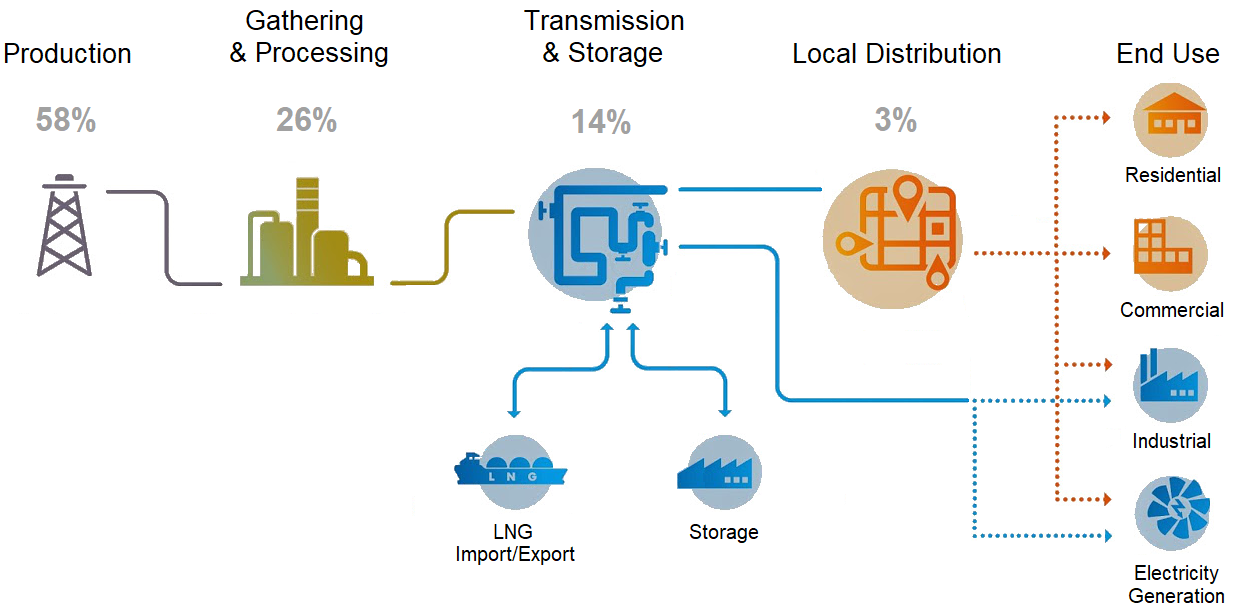
\includegraphics[width=\textwidth]{natural_gas_leakage_percentages_marks_fig1}

\textsc{Source:} \textcite{Marks:2021} figure~1, from estimates in \textcite{Alvarez/etal:2018}.
Excludes end-use leaks.
\end{figure}

\begin{table}[!bth]
\centering
\import{individual_figures/}{Cusworth_etal_2019_table2.tex}
\end{table}



\begin{figure}[!bth]
\caption{Distribution of detected methane leaks, comparison with ground-based measurement}
\label{fig:app-leak-sizes}
\includegraphics[width=0.49\textwidth]{leak_comparison_sizes}
\includegraphics[width=0.49\textwidth]{leak_comparison_fraction_with_detections}

\textsc{Left:} emissions conditional on detection.
\textsc{Right:} fraction of well pads with detected emissions.
The ``ground cens at'' columns are the ground studies' observations with artificial censoring applied, at either 5~or 10~kg/hr, the approximate detection threshold of both the California and Four Corners studies.
Without artificial censoring, the ground-based measurements are non-zero approximately 97\% of the time.
% Unrounded: 96.73913%
5~kg/hr is noted with a dashed line in the left plot.

\textsc{Sources:}
Ground studies include measurements primarily from
\textcite{Robertson/Edie/Snare/Soltis/Field/Burkhart/Bell/Zimmerle/Murphy:2017}
with additional contributions from
\textcite{
Rella/Tsai/Botkin/Crosson/Steele:2015,
Omara/Sullivan/Li/Subramanian/Robinson/Presto:2016,
Omara/Zimmerman/Sullivan/Li/Ellis/Cesa/Subramanian/Presto/Robinson:2018,
}.

California and Four Corners distributions come from aircraft studies \parencite{Duren/etal:2019, Frankenberg/etal:2016}.
\textcite{Lyon/Alvarez/Zavala-Araiza/Brandt/Jackson/Hamburg:2016}
provides information about leak prevalence (with a detection threshold roughly similar to the California and Four Corners studies), but not leak size.
\end{figure}



\begin{table}[!bth] % \ref{tab:covariate-balance-comparison}
\import{individual_figures/}{covariate_balance_comparison_detect_leak.tex}
\end{table}


\begin{figure}[!hbt] % \ref{fig:frankenberg-measurement-figs}
\import{individual_figures/}{frankenberg_measurement_figs.tex}
\end{figure}


\begin{figure}[!hbt] % \ref{fig:nat-gas-price-timeseries}
\import{individual_figures/}{nat_gas_price_timeseries.tex}
\end{figure}


\begin{figure}[!hbt] % \ref{fig:nat-gas-price-timeseries}
\caption{Matched natural gas prices exhibit little variation}
\label{fig:nat-gas-price-histogram}
\includegraphics[width=\textwidth]{nat_gas_price_histogram.pdf}
\end{figure}



\ifthenelse{\boolean{endfloat}}{}{\FloatBarrier} % add a \FloatBarrier if not using endfloat


\newpage

\section{Distribution Fitting}
\label{app:distribution-fitting}

\subsection{Model Priors}
\label{sec:model-priors}

We employ a fully Bayesian model, including priors on the parameters we estimate.
As noted in the main text, we choose priors that are very weakly informative on the outcome scale.
Specifically, we chose priors with mean zero and a standard deviation large enough that the predicted value of the outcomes \(e_i\) and \(q_i\) could take any reasonable value.
For \(e_i\), reasonable values are up to perhaps 100~times larger than the largest leak we see.
For \(q_i\), we aimed for a roughly uniform prior distribution by choosing priors of its underlying parameters.
The prior standard deviations are much smaller here;
because of the logit transformation, making the prior standard deviations larger would put a lot of prior weight on probabilities near zero or one
(see \cite{Gelman/etal:2020} for much more discussion).
We use a Student's \(t\) distribution with three degrees of freedom to allow for somewhat more weight in the distributions' tails than the Normal.
Specifically, we de-mean all of the \(X\) variables and use priors of
\(\text{generalized Student's } t(3, 0, 3)\) for each of the leak size parameters \(\beta\) and \(\sigma\).
We use \(\text{Normal}(0, 0.5)\) for the \(A_i\) coefficients \((\psi)\) and
\(\text{Normal}(0, 0.75)\) for the \(\alpha_i\) coefficients \((\phi)\).
While these seem like fairly narrow priors on first glance, these values lead to diffuse priors of the \(A_i\) and \(\alpha_i\).
After the inverse logit transformations described above, the priors on \((\psi)\) and \((\phi)\) are compatible with a wide range of values of  \(A_i\) and \(\alpha_i\).
The prior covariance between coefficients are all zero.

\subsection{Estimated Parameters}
\begin{table}[!bthp] % tab:model-param
\vspace*{-0.5\baselineskip}
\centering
\import{individual_figures/}{model_parameters.tex}
\end{table}


\begin{figure}[!bthp]
  \caption{Abatement elasticity \(-\hat{\alpha}_i\)}
  \label{fig:histogram-alphas}
  \includegraphics[width=0.99\textwidth]{model_cost_alpha_histogram}

Fitted values for \(\alpha_i\) from equation~\ref{eqn:alpha-fitted}.
Plot shows the distribution across wells, plotting the mean of across \gls{MCMC} draws of each \(\hat{\alpha_i}\).
Values are winsorized at the 99th percentile.
See discussion in section~\ref{sec:fitted-values}.
\end{figure}



\ifthenelse{\boolean{endfloat}}{}{\FloatBarrier} % add a \FloatBarrier if not using endfloat



\newpage
\section{Alternative Presentations of Policy Simulation Output}
\label{app:tabular-policy-output}

This section provides tabular versions of figures~\ref{fig:expected-fee-1pct} and \ref{fig:policy-outcomes-1pct}.
Please see those figures and the discussions in sections
\ref{sec:audit-probabilities-and-expected-fees} and
\ref{sec:dwl-and-emissions} for more description.
In these tables, bracketed values indicate 95\% \gls{CI}.

% \ref{tab:expected-fee-1pct}
\import{individual_figures/}{expected_fee_1pct_app_table.tex}


% \ref{tab:dwl-emis-1pct}
\import{individual_figures/}{policy_outcomes_dwl_emis_app_table_frac=1pct.tex}


\begin{figure}[!bthp]
  \caption{Curvature of \gls{DWL} and Emission Outcomes}
  \label{fig:policy-outcomes-1pct-cardinal}
  \includegraphics[width=\textwidth]{outcomes_dwl_emis_frac=1pct_cardinal}

This graph presents a version of the main-text figure~\ref{fig:policy-outcomes-1pct}, with x-axis values plotted on a cardinal scale, allowing the reader to have a better sense of the curvature of the \gls{DWL} and emissions outcomes at different fee levels.
This plot excludes the case of \(\tau \times T = \text{low} \times \text{3 months}\) for better visualization, as this case is fairly close to \(\tau \times T = \text{med} \times \text{1 week}\).
The plot includes two additional x-axis values, at \(\tau \times T = \) 2500 and 7500, chosen to improve coverage over the x-axis domain.
We present these additional points, rather than a smoother curve, because the computing required for each x-axis value is time-consuming.
\end{figure}

\ifthenelse{\boolean{endfloat}}{}{\FloatBarrier} % add a \FloatBarrier if not using endfloat


\newpage
\section{Drilling Response Details}
\label{app:drilling-response-details}

The main text considered the abatement behavior in a fixed population of wells.
However, charging additional fees and increasing abatement costs will make it less profitable to operate a well, and in equilibrium we expect the number of new wells drilled to decline.
This effect ends up being small relative to the per-well abatement.

First, we convert our methane leak fees into their approximate equivalent reduction in well profit from a change in prices.
Briefly, we total the well's expected fee payments and abatement costs, and find the change in commodity price that would result in an equivalent change to well profit, assuming the production quantity is unchanged.
Once we've calculated this price-equivalent change, we borrow supply and demand elasticities from the literature to estimate the change in drilling.
Both the profit-equivalent price change
(\import{tex_fragments/}{OUTCOME=net_private_cost_per_mcf_pct_price_RULE=target_e_high_FRAC=1pct_tauT=high-3month.tex}\%)
and the elasticity of drilling (0.36) are small, so this margin does not substantially affect our conclusions.

This calculation requires stronger assumptions than we applied in the main text.
We consider the extensive margin: wells that face some fee for their emissions will see lower profits, all else equal, than wells that face no fees.
Therefore, fewer wells will be drilled.
It is unlikely that existing wells will stop producing, or that wells will change the amount they produce \parencite{Anderson/Kellogg/Salant:2018}.
To keep things simple, we assume that there's no change in the composition of wells drilled.

To estimate an approximate drilling response, we first translate our expected fees into profit-equivalent changes in the price of natural gas, then we use estimates from the literature of the elasticity of drilling with respect to price.
Further, we assume that a well's cost of drilling does not change in this scenario, except for the cost of abatement.
We also assume that the policy does not lead to any change in the commodity price of natural gas.

To define some notation, say that without any methane policy a well operator spends \(D\) to drill a well, and implement the privately optimal level of abatement.
They earn \(E p_0\) revenue on the well's operation.
Here we elide complications like prices changing over time, uncertainty, and discounting.%
\footnote{%
Here we rely on a martingale price assumption, that today's price is the best guess for tomorrow's price.
Ignoring discounting is less of a problem than it would seem because we consider a change in price that applies to every future period, just as the expected change in profits applies in every future period.
}
With under an audit policy, they still spend \(D\) to drill the well, but now they also spend an additional \(C\) on abatement and \(F\) on expected fees.
Revenue is now \((E + \epsilon) p_0\), since some additional gas may be captured.
We define the profit-equivalent price change as the (lower) price that would result in the same profit the well would earn under the no-policy case.
The profit-equivalent price change is:
\[
\Delta p = \frac{C + F - \epsilon p_0}{E}
\]
For this calculation, we consider considering (\ref{policy-target-e}b), which uses remote measurements to target leaks and a realistic detection threshold.
Using the highest fee we considered (\(\tau = 2\delta\) and \(T\) = 3 months),
we find the production-weighted average price-equivalent is
\import{tex_fragments/}{OUTCOME=net_private_cost_per_mcf_pct_price_RULE=target_e_high_FRAC=1pct_tauT=high-3month.tex}\%
of the wholesale prices in our sample (which are approx. \$2.90--3.90).

For the price elasticity of drilling we rely on \textcite{Gilbert/Roberts:2020}, which calculates that the production-weighted long run elasticity of gas drilling with respect to the Henry Hub gas price is about 0.36 for all onshore drilling in the continental US, or 0.93 for their five-basin focus.
\footnote{%
In table 6 of that paper, the authors report the continental US short-run elasticity of 0.17 (s.e. 0.096), with the coefficient on the lagged dependent variable of 0.53 (s.e. 0.96).
We calculate the approximate long-run elasticity as 0.36 (\hbox{= 0.17 / (1 \(-\) 0.53)}).
}

Combining these, we come to the conclusion presented in the main text.
Even a high-fee policy would see at most a 5--10\% reduction in new (production weighted) drilling, and therefore the changes in expected emissions from this margin are small.

\section{Robustness to Alternative Sets of Variables}
\label{app:robustness-to-alternative-sets-of-variables}

As a robustness check of our specification, we run our analysis for the fee scenario of \(\tau \times T = \delta \times \text{3 months}\) using all subsets of our preferred set with at least two variables (56~specifications), plus combinations that use sub-basin fixed effects and inverse hyperbolic sine number of wells within 10~km (3~specifications \footnote{(1) our main
specification with basin dummies replaced by sub-basin cluster dummies, (2) our main
specification plus the number of wells within 10 km, and (3) both.}).


The sub-basin fixed effects are modeled by \gls{DBSCAN}, an unsupervised learning technique that assigns well pads to clusters and outliers.
\gls{DBSCAN} works by identifying clusters as regions of high density that are separated by regions of low density.
In contrast to counting the number of wells within a fixed radius, \gls{DBSCAN} can handle irregular geographic distributions of wells.
We used geospatial coordinates to cluster, and selected \gls{DBSCAN} parameters to provide subjectively reasonable-looking cluster patterns.
We end up with four clusters in the densely drilled San Joaquin basin, six in the rest of California, and one large cluster in the San Juan basin.
When we use these fixed effects in the regressions, we include one fixed effect level per cluster, and one level for each basin's outliers.
By including the sub-basin fixed effects and/or the number of wells within 10 km, our aim is to control for the well density information that was not accounted for in our preferred specification.

In figure~\ref{fig:robustness-reg-spec}, the preferred specification is in black and the other specifications are in gray.
The points for the preferred specification are qualitatively similar to the others. There are a few features to note here.
The range across specifications is quite narrow: roughly 10 percentage points from the lowest to the highest.
The confidence intervals here overlap substantially.
From these features, we conclude that our takeaways do not depend dramatically on the particular specification choice, at least among the variables included.



\begin{figure}[!bthp]
  \caption{Comparison across specifications}
  \label{fig:robustness-reg-spec}
  \includegraphics[width=\textwidth]{robustness_audit_result_dwl_rule=target_e_high_frac=1pct_tauT=med-3month}
  \includegraphics[width=\textwidth]{robustness_audit_result_emission_rule=target_e_high_frac=1pct_tauT=med-3month}

The top and bottom panels plot the change in \gls{DWL} and emissions for the case of \(\tau \times T = \delta \times \text{3 months}\).
The black point is our preferred specification
(see variables in table~\ref{tab:model-param}).
The gray points are alternative specifications, described in in appendix section~\ref{app:robustness-to-alternative-sets-of-variables}.
Bars indicate 95\% \gls{CI}.
To save computation resources, both the estimates and the confidence intervals are derived from standard \gls{MCMC} values, as opposed to the more computationally intensive BayesBag procedure employed in the main results of the paper.
These non-bootstrapped CIs are qualitatively similar to, and are slightly larger than, the bootstrapped CIs reported in figure~\ref{fig:policy-outcomes-1pct}.
\end{figure}


% Cites from the appendix:
% \printbibliography[heading=subbibliography, title={Appendix Citations}]
\end{refsection}

\newpage

\begin{refsection}[software_cites_r.bib,software_cites_python.bib]
\begin{RaggedRight}
\singlespacing
\twocolumn
\nocite{*}
\printbibliography[heading=subbibliography, title={Software Citations}]
\end{RaggedRight}
\end{refsection}
\end{document}
